\documentclass{amsart}
\usepackage{fullpage,graphicx,mathpazo,color}
\usepackage{amsmath,amscd,tikz,mathrsfs}
\usepackage[normalem]{ulem}
\usepackage{amsmath}
\usepackage{bm}
\usepackage{epstopdf}
\usepackage{tikz}
\usepackage{setspace}%ʹÓÃŒäŸàºê°ü
\usepackage{extarrows}
\usepackage{hyperref}
%\usepackage[backref]{hyperref}
%\usepackage[ctex]{ulem}
\newcommand{\ii}{\mathrm{i}}
\newcommand{\ee}{\mathrm{e}}
\newcommand{\dd}{\mathrm{d}}
\newcommand{\T}{\mathrm{T}}
\newcommand{\lm}[1]{{\color{red} #1}}
\newcommand{\xe}[1]{{\color{blue} #1}}

\newcommand{\cn}{\mathrm{cn}}
\newcommand{\sn}{\mathrm{sn}}
\newcommand{\dn}{\mathrm{dn}}
\newcommand{\Res}{\mathrm{Res}}


\newtheorem{rhp}{Riemann-Hilbert Problem}
\newtheorem{thm}{Theorem}
\newtheorem{lem}{Lemma}
\newtheorem{prop}{Proposition}
\newtheorem{corollary}{Corollary}
\newtheorem{definition}{Definition}
\newtheorem{conjecture}{Conjecture}
\newtheorem{rem}{Remark}
\newtheorem{example}{Example}

\usepackage{graphicx}      % insert graphic
% \usepackage{subcaption}
\usepackage{titlesec}
% \usepackage{graphicx}   % for \includegraphics
\usepackage{subcaption} % provides subfigure environment
\usepackage{caption}  
\usepackage{listings}
% optional: tell LaTeX where your figures live
\graphicspath{{figs/}}

\lstdefinestyle{matlabsmall}{
  language=Matlab,
  basicstyle=\ttfamily\scriptsize,
  keywordstyle=\color{blue},
  commentstyle=\color{gray},
  stringstyle=\color{red},
  numbers=left,
  numberstyle=\tiny,
  stepnumber=1,
  numbersep=5pt,
  breaklines=true,
  frame=single,
  columns=fullflexible,
  keepspaces=true,
  showstringspaces=false
}

\newcounter{hw}
\setcounter{hw}{0}

\numberwithin{equation}{hw}
\renewcommand{\theequation}{\thehw.\arabic{equation}}

\newcommand{\HW}[2]{%
  \refstepcounter{hw}%
  \setcounter{equation}{0}%
  \subsection*{HW \thehw: #1 \hfill {\small #2}}%
  \addcontentsline{toc}{section}{HW \thehw: #1 --- #2}%
}

% Define a better heading style for note sections
\newcommand{\noteheading}[1]{\vspace{1em}\noindent\textbf{#1}}

% Replace \paragraph with custom headings
% \newcommand{\obj}[1]{\noteheading{Objectives:} #1}
% \newcommand{\reading}[1]{\noteheading{Reading:} #1}
% \newcommand{\summary}{\noteheading{Lecture summary:}}
% \newcommand{\defs}{\noteheading{Definitions:}}
% \newcommand{\thms}{\noteheading{Theorems \& Propositions:}}
% \newcommand{\exs}{\noteheading{Examples:}}
% \newcommand{\exer}{\noteheading{Exercises:}}
% \newcommand{\notes}{\noteheading{Notes and remarks:}}
% \newcommand{\refs}{\noteheading{References:}}
% \newcommand{\extra}{\noteheading{Supplementary computations:}}



\titleformat{\section}{\centering\LARGE\bfseries}{\thesection}{1em}{}
\titleformat{\subsection}{\Large\bfseries}{\thesubsection}{1em}{}
\begin{document}


\title{Homeworks}

% \author{Liming Ling}
% \address{School of Mathematics, South China University of Technology, Guangzhou, China 510641}
% \email{linglm@scut.edu.cn}
\author{Zixuan Deng}
\address{School of Mathematics, South China University of Technology, Guangzhou}
\email{zxdengmath@163.com}

% \begin{abstract}
% These notes are based on the course \emph{Introduction to Integrable Systems}, delivered by Professor Liming Ling during the Fall semester of 2025--2026. 
% % They aim to provide a clear and structured exposition of the fundamental concepts, methods, and examples in the theory of integrable systems, serving both as a record of the lectures and as a reference for further study.

% The full \LaTeX{} source code of these notes is available at:  
% \href{https://codeberg.org/killlakill/courseNotes}{\texttt{https://codeberg.org/killlakill/courseNotes}}.

% \end{abstract}


\date{\today}

\maketitle


% ---------- Table of contents for a notes file ----------
% \begin{center}
%   \textbf{\large Course Notes (weekly)}\\[4pt]
%   \textit{--- Table of Contents (auto-generated) ---}
% \end{center}
% \smallskip
% \tableofcontents
% \bigskip
% \hrule
% \bigskip


\HW{Two-Step Gauge Transformation}{2026-04-22}



% \summary{Starting from the Lax pair, we expand the formal solution, obtain recursive relations for the coefficients, and use them to derive the evolution equations. This yields the mKdV equation as a member of the AKNS hierarchy, with all steps carried out explicitly.} 


Consider the system
\begin{align}
\mathrm{i}\Psi_t
&=
\frac{1}{2}Q^2\Psi
-
(\Psi^\dagger\Psi)\Psi
+
\frac{\Delta}{2}\sigma_3\Psi,
\qquad
\Psi=(\Psi_1,\Psi_2)^\top,
\label{eq:initial-system}
\\
Q
&=
-\mathrm{i}\partial_x+\alpha A(x),
\qquad
A(x)
=
\begin{pmatrix}
0 & {\mathrm e}^{-2\mathrm{i}kx}
\\
{\mathrm e}^{2\mathrm{i}kx} & 0
\end{pmatrix}.
\label{eq:A-matrix}
\end{align}
Here
\begin{equation}
\sigma_1=
\begin{pmatrix}
0 & 1\\
1 & 0
\end{pmatrix},
\qquad
\sigma_2=
\begin{pmatrix}
0 & -\mathrm{i}\\
\mathrm{i} & 0
\end{pmatrix},
\qquad
\sigma_3=
\begin{pmatrix}
1 & 0\\
0 & -1
\end{pmatrix}
\label{eq:pauli-matrices}
\end{equation}
denote the Pauli matrices.

We first compute the square of $Q$. Since
\begin{equation}
A(x)^2=\mathbb{I}_2,
\qquad
A_x(x)=
\begin{pmatrix}
0 & -2\mathrm{i}k\,{\mathrm e}^{-2\mathrm{i}kx}
\\
2\mathrm{i}k\,{\mathrm e}^{2\mathrm{i}kx} & 0
\end{pmatrix},
\label{eq:A-square}
\end{equation}
we obtain
\begin{align}
Q^2
&=
\bigl(-\mathrm{i}\partial_x+\alpha A\bigr)^2
\nonumber\\
&=
-\partial_x^2
-\mathrm{i}\alpha A\partial_x
-\mathrm{i}\alpha\partial_x(A\,\cdot)
+\alpha^2A^2
\nonumber\\
&=
-\partial_x^2
-\mathrm{i}\alpha A\partial_x
-\mathrm{i}\alpha(A_x+A\partial_x)
+\alpha^2A^2
\nonumber\\
&=
-\partial_x^2
-2\mathrm{i}\alpha A\partial_x
-\mathrm{i}\alpha A_x
+\alpha^2.
\label{eq:Q-square}
\end{align}
Substituting \eqref{eq:Q-square} into \eqref{eq:initial-system} yields
\begin{equation}
\mathrm{i}\Psi_t
=
-\frac{1}{2}\Psi_{xx}
-\mathrm{i}\alpha A\Psi_x
-\frac{\mathrm{i}}{2}\alpha A_x\Psi
+\frac{1}{2}\alpha^2\Psi
-|\Psi|^2\Psi
+\frac{\Delta}{2}\sigma_3\Psi.
\label{eq:expanded-system}
\end{equation}

Define the gauge transformation
\begin{equation}
\Psi(x,t)
=
\Lambda(x,t)\psi(x,t),
\qquad
\Lambda(x,t)
=
{\mathrm e}^{-\frac{\mathrm{i}}{2}(\alpha^2+k^2)t}
{\mathrm e}^{-\mathrm{i}kx\sigma_3}.
\label{eq:first-gauge}
\end{equation}
Since $\sigma_3^2=\mathbb{I}_2$, the matrix exponential may be written as
\begin{equation}
{\mathrm e}^{-\mathrm{i}kx\sigma_3}
=
\begin{pmatrix}
{\mathrm e}^{-\mathrm{i}kx} & 0
\\
0 & {\mathrm e}^{\mathrm{i}kx}
\end{pmatrix},
\end{equation}
and therefore $\Lambda$ is unitary:
\begin{equation}
\Lambda^\dagger\Lambda=\mathbb{I}_2.
\label{eq:Lambda-unitary}
\end{equation}
Consequently,
\begin{equation}
|\Psi|^2
=
\Psi^\dagger\Psi
=
\psi^\dagger\Lambda^\dagger\Lambda\psi
=
\psi^\dagger\psi
=
|\psi|^2.
\label{eq:norm-invariant}
\end{equation}

Differentiating \eqref{eq:first-gauge} gives
\begin{equation}
\Lambda_t
=
-\frac{\mathrm{i}}{2}(\alpha^2+k^2)\Lambda,
\qquad
\Lambda_x
=
-\mathrm{i}k\sigma_3\Lambda.
\label{eq:Lambda-derivatives}
\end{equation}
Hence
\begin{align}
\Psi_t
&=
\Lambda_t\psi+\Lambda\psi_t
=
\Lambda\left(
-\frac{\mathrm{i}}{2}(\alpha^2+k^2)\psi+\psi_t
\right),
\label{eq:Psi-t}
\\
\Psi_x
&=
\Lambda_x\psi+\Lambda\psi_x
=
\Lambda\left(
-\mathrm{i}k\sigma_3\psi+\psi_x
\right),
\label{eq:Psi-x}
\end{align}
and
\begin{align}
\Psi_{xx}
&=
\partial_x\!\left[
\Lambda\left(
-\mathrm{i}k\sigma_3\psi+\psi_x
\right)
\right]
\nonumber\\
&=
\Lambda_x\left(
-\mathrm{i}k\sigma_3\psi+\psi_x
\right)
+
\Lambda\left(
-\mathrm{i}k\sigma_3\psi_x+\psi_{xx}
\right)
\nonumber\\
&=
\Lambda\left[
-\mathrm{i}k\sigma_3
\left(
-\mathrm{i}k\sigma_3\psi+\psi_x
\right)
-\mathrm{i}k\sigma_3\psi_x
+\psi_{xx}
\right]
\nonumber\\
&=
\Lambda\left(
-k^2\psi
-2\mathrm{i}k\sigma_3\psi_x
+\psi_{xx}
\right).
\label{eq:Psi-xx}
\end{align}

Next we compute the conjugation of $A(x)$ by $\Lambda$. Since the scalar phase
\(
{\mathrm e}^{-\frac{\mathrm{i}}{2}(\alpha^2+k^2)t}
\)
commutes with every matrix, we have
\begin{align}
\Lambda^{-1}A(x)\Lambda
&=
{\mathrm e}^{\mathrm{i}kx\sigma_3}
A(x)
{\mathrm e}^{-\mathrm{i}kx\sigma_3}
\nonumber\\
&=
\begin{pmatrix}
{\mathrm e}^{\mathrm{i}kx} & 0
\\
0 & {\mathrm e}^{-\mathrm{i}kx}
\end{pmatrix}
\begin{pmatrix}
0 & {\mathrm e}^{-2\mathrm{i}kx}
\\
{\mathrm e}^{2\mathrm{i}kx} & 0
\end{pmatrix}
\begin{pmatrix}
{\mathrm e}^{-\mathrm{i}kx} & 0
\\
0 & {\mathrm e}^{\mathrm{i}kx}
\end{pmatrix}
\nonumber\\
&=
\begin{pmatrix}
0 & 1
\\
1 & 0
\end{pmatrix}
=
\sigma_1.
\label{eq:A-conjugation}
\end{align}
Similarly,
\begin{align}
\Lambda^{-1}A_x(x)\Lambda
=
\begin{pmatrix}
0 & -2\mathrm{i}k
\\
2\mathrm{i}k & 0
\end{pmatrix}
=
2k
\begin{pmatrix}
0 & -\mathrm{i}
\\
\mathrm{i} & 0
\end{pmatrix}
=
2k\sigma_2
=
2\mathrm{i}k\sigma_1\sigma_3.
\label{eq:Ax-conjugation}
\end{align}
Moreover,
\begin{equation}
\Lambda^{-1}\sigma_3\Lambda
=
\sigma_3,
\label{eq:sigma3-conjugation}
\end{equation}
since $\sigma_3$ commutes with ${\mathrm e}^{-\mathrm{i}kx\sigma_3}$.

Substituting \eqref{eq:Psi-t}, \eqref{eq:Psi-x}, and \eqref{eq:Psi-xx} into \eqref{eq:expanded-system}, we obtain
\begin{align}
&\mathrm{i}\Lambda
\left(
-\frac{\mathrm{i}}{2}(\alpha^2+k^2)\psi+\psi_t
\right)
\nonumber\\
&=
-\frac12
\Lambda
\left(
-k^2\psi
-2\mathrm{i}k\sigma_3\psi_x
+\psi_{xx}
\right)
\nonumber\\
&\quad
-\mathrm{i}\alpha A\Lambda
\left(
-\mathrm{i}k\sigma_3\psi+\psi_x
\right)
-\frac{\mathrm{i}}{2}\alpha A_x\Lambda\psi
+\frac12\alpha^2\Lambda\psi
\nonumber\\
&\quad
-|\psi|^2\Lambda\psi
+\frac{\Delta}{2}\sigma_3\Lambda\psi.
\label{eq:substituted-system}
\end{align}
Multiplying \eqref{eq:substituted-system} from the left by $\Lambda^{-1}$ and using
\eqref{eq:A-conjugation}--\eqref{eq:sigma3-conjugation} gives
\begin{align}
\frac12(\alpha^2+k^2)\psi+\mathrm{i}\psi_t
&=
\frac12k^2\psi
+\mathrm{i}k\sigma_3\psi_x
-\frac12\psi_{xx}
\nonumber\\
&\quad
-\mathrm{i}\alpha\sigma_1
\left(
-\mathrm{i}k\sigma_3\psi+\psi_x
\right)
-\mathrm{i}\alpha k\sigma_2\psi
\nonumber\\
&\quad
+\frac12\alpha^2\psi
-|\psi|^2\psi
+\frac{\Delta}{2}\sigma_3\psi.
\label{eq:before-cancellation}
\end{align}
Using the identity
\begin{equation}
\sigma_1\sigma_3=-\mathrm{i}\sigma_2,
\label{eq:pauli-identity}
\end{equation}
we find
\begin{equation}
-\mathrm{i}\alpha\sigma_1(-\mathrm{i}k\sigma_3\psi)
=
\mathrm{i}\alpha k\sigma_2\psi,
\end{equation}
which exactly cancels the term
\(
-\mathrm{i}\alpha k\sigma_2\psi
\)
in \eqref{eq:before-cancellation}. After cancellation of the constant terms, we arrive at
\begin{equation}
\mathrm{i}\psi_t
=
-\frac12\psi_{xx}
+\mathrm{i}(k\sigma_3-\alpha\sigma_1)\psi_x
-|\psi|^2\psi
+\frac{\Delta}{2}\sigma_3\psi.
\label{eq:first-transformed-system}
\end{equation}


We now introduce the second gauge transformation
\begin{equation}
\psi(x,t)
=
V(x,t)q(x,t),
\qquad
V(x,t)
=
{\mathrm e}^{\frac{\mathrm{i}}{2}(\alpha^2+k^2)t}\,
B\,
{\mathrm e}^{-\mathrm{i}\kappa x\sigma_3},
\qquad
\kappa=\sqrt{\alpha^2+k^2},
\label{eq:second-gauge}
\end{equation}
where
\begin{equation}
B=
\begin{pmatrix}
-\sin\varphi & -\cos\varphi
\\
\cos\varphi & -\sin\varphi
\end{pmatrix}
=
-\sin\varphi\,\mathbb{I}_2
+
\cos\varphi\,\sigma_1\sigma_3.
\label{eq:B-matrix}
\end{equation}

The angle $\varphi$ is chosen so that
\begin{equation}
2\varphi
=
\arctan\frac{k}{\alpha}-\frac{\pi}{2}.
\label{eq:phi-definition}
\end{equation}
Hence
\begin{equation}
\tan(2\varphi)
=
-\frac{\alpha}{k},
\end{equation}
and therefore
\begin{equation}
\sin(2\varphi)
=
-\frac{\alpha}{\sqrt{\alpha^2+k^2}},
\qquad
\cos(2\varphi)
=
\frac{k}{\sqrt{\alpha^2+k^2}}.
\label{eq:trig-identities}
\end{equation}

Since $B$ is independent of $x$ and $t$, differentiating
\eqref{eq:second-gauge} yields
\begin{align}
\psi_t
&=
V
\left(
\frac{\mathrm{i}}{2}\kappa^2q+q_t
\right),
\label{eq:psi-t-q}
\\
\psi_x
&=
V
\left(
-\mathrm{i}\kappa\sigma_3q+q_x
\right),
\label{eq:psi-x-q}
\\
\psi_{xx}
&=
V
\left(
-\kappa^2q
-2\mathrm{i}\kappa\sigma_3q_x
+q_{xx}
\right).
\label{eq:q-derivatives}
\end{align}

Next we compute several algebraic identities associated with $B$. Since
\begin{equation}
B^\top
=
\begin{pmatrix}
-\sin\varphi & \cos\varphi
\\
-\cos\varphi & -\sin\varphi
\end{pmatrix},
\end{equation}
a direct computation gives
\begin{equation}
B^\top B
=
\mathbb{I}_2.
\label{eq:B-orthogonal}
\end{equation}
Consequently,
\begin{equation}
V^\dagger V
=
\mathbb{I}_2,
\end{equation}
and hence the nonlinear term is preserved:
\begin{equation}
|\psi|^2
=
\psi^\dagger\psi
=
q^\dagger V^\dagger V q
=
q^\dagger q
=
|q|^2.
\label{eq:q-norm}
\end{equation}

We now compute the conjugation of $\sigma_3$ by $B$. Using
\eqref{eq:trig-identities}, one finds
\begin{align}
B^\top\sigma_3B
=
\begin{pmatrix}
-\cos(2\varphi) & \sin(2\varphi)
\\
\sin(2\varphi) & \cos(2\varphi)
\end{pmatrix}
=
-\frac{1}{\sqrt{\alpha^2+k^2}}
\begin{pmatrix}
k & \alpha
\\
\alpha & -k
\end{pmatrix}.
\label{eq:B-conjugation}
\end{align}

Using
\eqref{eq:B-matrix}, we compute
\begin{align}
B^\top(k\sigma_3-\alpha\sigma_1)B
&=
kB^\top\sigma_3B-\alpha B^\top\sigma_1B
\nonumber\\
&=
\begin{pmatrix}
-k\cos(2\varphi)+\alpha\sin(2\varphi)
&
k\sin(2\varphi)+\alpha\cos(2\varphi)
\\
k\sin(2\varphi)+\alpha\cos(2\varphi)
&
k\cos(2\varphi)-\alpha\sin(2\varphi)
\end{pmatrix}.
\end{align}
Substituting \eqref{eq:trig-identities} gives
\begin{equation}
B^\top(k\sigma_3-\alpha\sigma_1)B
=
\begin{pmatrix}
-\kappa & 0
\\
0 & \kappa
\end{pmatrix}
=
-\kappa\sigma_3.
\label{eq:B-diagonalization}
\end{equation}

Substituting \eqref{eq:psi-t-q}--\eqref{eq:q-derivatives} into
\eqref{eq:first-transformed-system}, we obtain
\begin{align}
\mathrm{i}V
\left(
\frac{\mathrm{i}}{2}\kappa^2q+q_t
\right)
&=
-\frac12
V
\left(
-\kappa^2q
-2\mathrm{i}\kappa\sigma_3q_x
+q_{xx}
\right)
\nonumber\\
&\quad
+
\mathrm{i}(k\sigma_3-\alpha\sigma_1)
V
\left(
-\mathrm{i}\kappa\sigma_3q+q_x
\right)
-|q|^2Vq
+\frac{\Delta}{2}\sigma_3Vq.
\label{eq:q-substitution}
\end{align}
Multiplying \eqref{eq:q-substitution} from the left by $V^{-1}$ yields
\begin{align}
-\frac12\kappa^2q+\mathrm{i}q_t
&=
\frac12\kappa^2q
+\mathrm{i}\kappa\sigma_3q_x
-\frac12q_{xx}
\nonumber\\
&\quad
+
\mathrm{i}V^{-1}(k\sigma_3-\alpha\sigma_1)V
\left(
-\mathrm{i}\kappa\sigma_3q+q_x
\right)
\nonumber\\
&\quad
-|q|^2q
+\frac{\Delta}{2}V^{-1}\sigma_3Vq.
\label{eq:q-before-cancel}
\end{align}

Since
\begin{equation}
V^{-1}(k\sigma_3-\alpha\sigma_1)V
=
{\mathrm e}^{\mathrm{i}\kappa x\sigma_3}
B^\top(k\sigma_3-\alpha\sigma_1)B
{\mathrm e}^{-\mathrm{i}\kappa x\sigma_3},
\end{equation}
equation \eqref{eq:B-diagonalization} implies
\begin{equation}
V^{-1}(k\sigma_3-\alpha\sigma_1)V
=
-\kappa\sigma_3.
\label{eq:diagonalized-operator}
\end{equation}
Substituting \eqref{eq:diagonalized-operator} into
\eqref{eq:q-before-cancel}, the first-order derivative terms cancel:
\begin{align}
\mathrm{i}q_t
&=
-\frac12q_{xx}
-|q|^2q
+\frac{\Delta}{2}V^{-1}\sigma_3Vq.
\label{eq:q-equation-pre-final}
\end{align}

Finally,
\begin{align}
V^{-1}\sigma_3V
&=
{\mathrm e}^{\mathrm{i}\kappa x\sigma_3}
B^\top\sigma_3B
{\mathrm e}^{-\mathrm{i}\kappa x\sigma_3}
\nonumber\\
&=
{\mathrm e}^{\mathrm{i}\kappa x\sigma_3}
\frac{-1}{\sqrt{\alpha^2+k^2}}
\begin{pmatrix}
k & \alpha
\\
\alpha & -k
\end{pmatrix}
{\mathrm e}^{-\mathrm{i}\kappa x\sigma_3}.
\label{eq:sigma3-final-transform}
\end{align}
Therefore,
\begin{align}
\mathrm{i}q_t
&=
-\frac{1}{2}q_{xx}
-|q|^2q
+\frac{\Delta}{2}
{\mathrm e}^{\mathrm{i}\kappa x\sigma_3}
\frac{-1}{\sqrt{\alpha^2+k^2}}
\begin{pmatrix}
k & \alpha
\\
\alpha & -k
\end{pmatrix}
{\mathrm e}^{-\mathrm{i}\kappa x\sigma_3}q.
\label{eq:final-system}
\end{align}


\HW{The squared eigenfunctions on Weierstrass points}{2026-04-29}

Let \(B\in\mathbb{C}^{g\times g}\) be a symmetric matrix with positive definite imaginary part. The associated Riemann theta function is defined by
\begin{equation}
\Theta(\bm{z},B)
=
\sum_{\bm{n}\in\mathbb{Z}^{g}}
\exp\!\left(
\pi\mathrm{i}\,\bm{n}^{\top}B\bm{n}
+
2\pi\mathrm{i}\,\bm{n}^{\top}\bm{z}
\right),
\qquad
\bm{z}\in\mathbb{C}^{g}.
\label{eq:Riemann-theta}
\end{equation}

For \(k=1,\ldots,g\), let
\[
\bm{e}_k
=
(0,\ldots,0,1,0,\ldots,0)^{\top}
\]
denote the \(k\)-th standard basis vector of \(\mathbb{R}^{g}\). The theta function satisfies the quasi-periodicity relations
\begin{equation}
\Theta(\bm{z}+\bm{e}_k,B)
=
\Theta(\bm{z},B),
\label{eq:theta-periodicity-1}
\end{equation}
and
\begin{equation}
\Theta(\bm{z}+B\bm{e}_k,B)
=
\exp\!\left(
-2\pi\mathrm{i}\,z_k
-
\pi\mathrm{i}\,B_{kk}
\right)
\Theta(\bm{z},B),
\label{eq:theta-periodicity-2}
\end{equation}
where \(z_k\) denotes the \(k\)-th component of \(\bm{z}\).

Consider the genus-two hyperelliptic curve
\begin{equation}
\mathscr{F}_2
=
\left\{
P=(\lambda,y)
\;\middle|\;
y^2
=
\prod_{j=1}^{3}
(\lambda-\lambda_j)(\lambda-\lambda_j^*)
\right\},
\label{eq:genus-two-curve}
\end{equation}
with \(\lambda\in\mathbb{CP}^1\).

In Case~1, we assume that
\[
\lambda_1,\lambda_2,\lambda_3\in \mathrm{i}\mathbb{R},
\qquad
\Im \lambda_3>\Im \lambda_2>\Im \lambda_1>0 .
\]

Let \(\{a_1,a_2,b_1,b_2\}\) be a canonical homology basis satisfying
\[
a_i\circ b_j
=
-
b_j\circ a_i
=
\delta_{ij},
\qquad
a_i\circ a_j
=
0,
\qquad
b_i\circ b_j
=
0 .
\]
Let \(\{w_1\,d\lambda,w_2\,d\lambda\}\) be the normalized basis of holomorphic differentials determined by
\begin{equation}
\oint_{a_j} w_i\,d\lambda
=
\delta_{ij},
\qquad
\oint_{b_j} w_i\,d\lambda
=
B_{ij},
\label{eq:normalized-differentials}
\end{equation}
for \(i,j=1,2\).

For a fixed base point \(P_0\in\mathscr{F}_2\), the Abel map is defined by
\begin{equation}
\mathcal{A}_{P_0}(P)
=
\bigl(
\mathcal{A}_{P_0,1}(P),
\mathcal{A}_{P_0,2}(P)
\bigr)^{\top}
=
\Biggl(
\int_{P_0}^{P} w_1\,d\lambda,
\;
\int_{P_0}^{P} w_2\,d\lambda
\Biggr)^{\top}.
\label{eq:Abel-map}
\end{equation}

Let \(d\Omega_1,d\Omega_2,d\Omega_3\) be normalized Abelian differentials satisfying
\begin{equation}
\oint_{a_j} d\Omega_k
=
0,
\qquad
j=1,2,
\quad
k=1,2,3.
\label{eq:a-normalization}
\end{equation}
Their corresponding Abelian integrals admit the asymptotic expansions
\begin{equation}
\Omega_1(P)
=
\pm\left(
\ln \lambda
+
\ln \omega_1
+
o(1)
\right),
\qquad
P\to\infty^\pm,
\label{eq:Omega1-asymptotic}
\end{equation}
\begin{equation}
\Omega_2(P)
=
\pm\left(
\lambda
+
\omega_2
+
o(1)
\right),
\qquad
P\to\infty^\pm,
\label{eq:Omega2-asymptotic}
\end{equation}
and
\begin{equation}
\Omega_3(P)
=
\pm\left(
2\lambda^2
+
\omega_3
+
o(1)
\right),
\qquad
P\to\infty^\pm.
\label{eq:Omega3-asymptotic}
\end{equation}

Fix the base point \(P_0=(\lambda_3,0)\), and define
\begin{equation}
\Omega_k(P)
=
\int_{P_0}^{P} d\Omega_k,
\qquad
k=1,2,3.
\label{eq:Omega-definition}
\end{equation}

The corresponding \(b\)-period vectors are defined by
\begin{equation}
U_k
=
\frac{1}{2\pi\mathrm{i}}
\oint_{b_k} d\Omega_2,
\qquad
V_k
=
\frac{1}{2\pi\mathrm{i}}
\oint_{b_k} d\Omega_3,
\qquad
\Delta_k
=
-
\frac{1}{2\pi\mathrm{i}}
\oint_{b_k} d\Omega_1,
\label{eq:period-vectors}
\end{equation}
for \(k=1,2\). If \(\ell\) is a positively oriented circle surrounding \(\infty^+\), then
\begin{equation}
\oint_{\ell} d\Omega_1
=
2\pi\mathrm{i}.
\label{eq:Omega1-cycle}
\end{equation}

The vectors \(U=(U_1,U_2)\) and \(V=(V_1,V_2)\) satisfy
\begin{equation}
U_1
=
U_2
\in
\mathrm{i}\mathbb{R},
\label{eq:U-reality}
\end{equation}
and
\begin{equation}
V_1
=
-
V_2
\in
\mathbb{R}.
\label{eq:V-reality}
\end{equation}
Moreover,
\begin{equation}
\Delta_k\in\mathbb{R},
\qquad
\Delta_1+\Delta_2=1,
\label{eq:reality-conditions}
\end{equation}
and the symmetry relation
\begin{equation}
\sigma_1\Delta
=
-
\Delta
+
\bm{1},
\qquad
\bm{1}
=
\begin{pmatrix}
1\\
1
\end{pmatrix},
\qquad
\sigma_1
=
\begin{pmatrix}
0 & 1\\
1 & 0
\end{pmatrix},
\label{eq:Delta-symmetry}
\end{equation}
holds.

Define
\begin{equation}
\Omega
=
D+\mathrm{i}Ux+\mathrm{i}Vt
=
\mathrm{i}U(x-x_0)+\mathrm{i}V(t-t_0),
\label{eq:Omega-vector}
\end{equation}
where \(D=-\mathrm{i}Ux_0-\mathrm{i}Vt_0\), and let
\begin{equation}
\Delta
=
\mathcal{A}_{P_0}(\infty^+)
-
\mathcal{A}_{P_0}(\infty^-)
=
\mathcal{A}_{\infty^-}(\infty^+).
\label{eq:Delta-divisor}
\end{equation}
Then
\begin{equation}
\sigma_1\Omega^*
=
\Omega,
\qquad
\mathcal{A}_{\infty^-}(P_0)
=
\frac{\Delta}{2},
\qquad
\mathcal{A}_{\infty^+}(P_0)
=
-
\frac{\Delta}{2}.
\label{eq:Abel-symmetry}
\end{equation}

The Baker--Akhiezer function associated with the two-phase solution is given by
\begin{equation}
\begin{pmatrix}
\Phi_{11}(P;x,t)\\[4pt]
\Phi_{21}(P;x,t)
\end{pmatrix}
=
\exp\!\left[
-
\mathrm{i}
\left(
\omega_2x+\omega_3t+\frac{\theta}{2}
+\frac{\mathrm{i}}{2}\Omega_1(P)
\right)
\sigma_3
\right]
\begin{pmatrix}
\Theta\bigl(\Omega+\mathcal{A}_{\infty^+}(P)\bigr)\\[4pt]
\Theta\bigl(\Omega+\Delta+\mathcal{A}_{\infty^+}(P)\bigr)
\end{pmatrix}
\frac{
\exp\!\bigl(
\mathrm{i}\Omega_2(P)x
+
\mathrm{i}\Omega_3(P)t
\bigr)
}{
\Theta(\Omega)
}.
\label{eq:BA-function}
\end{equation}
Here \(\omega_2=0\) and \(\omega_3\in\mathbb{R}\).

Using \eqref{eq:Abel-symmetry}, we obtain
\begin{equation}
\Omega+\mathcal{A}_{\infty^+}(P)
=
\Omega
-
\frac{\Delta}{2}
+
\mathcal{A}_{P_0}(P),
\label{eq:shift-plus}
\end{equation}
and
\begin{equation}
\Omega+\Delta+\mathcal{A}_{\infty^+}(P)
=
\Omega
+
\frac{\Delta}{2}
+
\mathcal{A}_{P_0}(P).
\label{eq:shift-minus}
\end{equation}


Define the branch points
\begin{equation}
P_j
=
(\lambda_j,0),
\qquad
P_{-j}
=
(\lambda_j^*,0),
\qquad
j=1,2,3.
\label{eq:branch-points}
\end{equation}

For \(P\in\mathscr{F}_2\), define
\begin{equation}
\bm{P}_1(P)
=
\begin{pmatrix}
\Phi_{11}(P)\\[4pt]
\Phi_{21}(P)
\end{pmatrix}
\begin{pmatrix}
\Phi_{11}^*\bigl(\tau_R(\iota(P))\bigr),
&
\Phi_{21}^*\bigl(\tau_R(\iota(P))\bigr)
\end{pmatrix},
\label{eq:P1-definition}
\end{equation}
and
\begin{equation}
\bm{S}_1(P)
=
\begin{pmatrix}
\Phi_{21}(P)\,
\Phi_{11}^*\bigl(\tau_R(\iota(P))\bigr)
\\[6pt]
\Phi_{11}(P)\,
\Phi_{21}^*\bigl(\tau_R(\iota(P))\bigr)
\end{pmatrix}.
\label{eq:S1-definition}
\end{equation}

Here \(\tau_R\) and \(\iota\) denote the involutions
\begin{equation}
\tau_R:(\lambda,y)\mapsto(\lambda^*,y^*),
\qquad
\iota:(\lambda,y)\mapsto(\lambda,-y).
\label{eq:involutions}
\end{equation}

Let
\begin{equation}
\mathscr{P}:\mathscr{F}_2\to\mathbb{CP}^1,
\qquad
\mathscr{P}(\lambda,y)=\lambda,
\label{eq:projection-map}
\end{equation}
be the canonical projection map. We consider \(\bm{S}_1(P)\) at the Weierstrass points satisfying
\[
\mathscr{P}(P)
=
\pm\lambda_1,
\pm\lambda_2,
\pm\lambda_3.
\]

Since \(P\) is a branch point, one has \(\iota(P)=P\). Hence
\begin{equation}
\bm{S}_1(P)
=
\begin{pmatrix}
\Phi_{21}(P)\,
\Phi_{11}^*\bigl(\tau_R(P)\bigr)
\\[6pt]
\Phi_{11}(P)\,
\Phi_{21}^*\bigl(\tau_R(P)\bigr)
\end{pmatrix}.
\label{eq:S1-branch-points}
\end{equation}

We now establish the following result concerning the squared eigenfunctions evaluated at the Weierstrass points.

\begin{prop}\label{prop:hw2}
The vectors
\[
\bm{S}_1(P_j),
\qquad
j=\pm1,\pm2,\pm3,
\]
span a three-dimensional subspace. More precisely,
\begin{equation}
\dim
\Bigl(
\operatorname{span}
\{
\bm{S}_1(P_j)
:\,
j=\pm1,\pm2,\pm3
\}
\Bigr)
=
3.
\label{eq:span-dimension-prop}
\end{equation}
\end{prop}


Define
\begin{equation}
\begin{pmatrix}
\widetilde{\Phi}_{11}(P)\\[4pt]
\widetilde{\Phi}_{21}(P)
\end{pmatrix}
=
\exp\!\left[
-
\mathrm{i}
\left(
\omega_2x+\omega_3t+\frac{\theta}{2}
+\frac{\mathrm{i}}{2}\Omega_1(P)
\right)
\sigma_3
\right]
\begin{pmatrix}
\Theta\!\left(
\Omega-\dfrac{\Delta}{2}
+\mathcal{A}_{P_0}(P)
\right)
\\[8pt]
\Theta\!\left(
\Omega+\dfrac{\Delta}{2}
+\mathcal{A}_{P_0}(P)
\right)
\end{pmatrix}.
\label{eq:tilde-Phi}
\end{equation}

Taking complex conjugates at the reflected point \(\tau_R(P)\), we obtain
\begin{align}
&
\begin{pmatrix}
\widetilde{\Phi}_{11}^*\bigl(\tau_R(P)\bigr)
&
\widetilde{\Phi}_{21}^*\bigl(\tau_R(P)\bigr)
\end{pmatrix}
\nonumber\\[4pt]
&=
\begin{pmatrix}
\Theta^*\!\left(
\Omega-\dfrac{\Delta}{2}
+\mathcal{A}_{P_0}\bigl(\tau_R(P)\bigr)
\right),
&
\Theta^*\!\left(
\Omega+\dfrac{\Delta}{2}
+\mathcal{A}_{P_0}\bigl(\tau_R(P)\bigr)
\right)
\end{pmatrix}
\nonumber\\[4pt]
&\hspace{2cm}\times
\exp\!\left[
\mathrm{i}
\left(
\omega_2x+\omega_3t+\frac{\theta}{2}
-
\frac{\mathrm{i}}{2}\Omega_1^*\bigl(\tau_R(P)\bigr)
\right)
\sigma_3
\right].
\label{eq:tilde-Phi-conjugate}
\end{align}

Substituting these expressions into the definition of \(\bm{S}_1(P)\) yields
\begin{equation}
\bm{S}_1(P)
=
\widetilde{\bm{S}}_1(P)
\frac{
\exp\!\left(
\mathrm{i}
\bigl(
\Omega_2(P)-\Omega_2^*(\tau_R(P))
\bigr)x
+
\mathrm{i}
\bigl(
\Omega_3(P)-\Omega_3^*(\tau_R(P))
\bigr)t
\right)
}{
|\Theta(\Omega)|^2
}.
\label{eq:S1-factorization}
\end{equation}
Here
\begin{equation}
\widetilde{\bm{S}}_1(P)
=
\begin{pmatrix}
\widetilde{\Phi}_{21}(P)\,
\widetilde{\Phi}_{11}^*\bigl(\tau_R(P)\bigr)
\\[8pt]
\widetilde{\Phi}_{11}(P)\,
\widetilde{\Phi}_{21}^*\bigl(\tau_R(P)\bigr)
\end{pmatrix}.
\label{eq:tilde-S1}
\end{equation}

Using \eqref{eq:tilde-Phi} and \eqref{eq:tilde-Phi-conjugate}, we further obtain
\begin{align}
\widetilde{\bm{S}}_1(P)
&=
\exp\!\left[
\mathrm{i}
\left(
2\omega_2x
+
2\omega_3t
+
\theta
+
\frac{\mathrm{i}}{2}
\bigl(
\Omega_1(P)-\Omega_1^*\bigl(\tau_R(P)\bigr)
\bigr)
\right)
\sigma_3
\right]
\nonumber\\[4pt]
&\quad\times
\begin{pmatrix}
\Theta\!\left(
\Omega+\dfrac{\Delta}{2}
+\mathcal{A}_{P_0}(P)
\right)
\Theta^*\!\left(
\Omega-\dfrac{\Delta}{2}
+\mathcal{A}_{P_0}\bigl(\tau_R(P)\bigr)
\right)
\\[10pt]
\Theta\!\left(
\Omega-\dfrac{\Delta}{2}
+\mathcal{A}_{P_0}(P)
\right)
\Theta^*\!\left(
\Omega+\dfrac{\Delta}{2}
+\mathcal{A}_{P_0}\bigl(\tau_R(P)\bigr)
\right)
\end{pmatrix}.
\label{eq:tilde-S1-expanded}
\end{align}

Since
\begin{equation}
\mathcal{A}_{P_0}(P)
=
\begin{pmatrix}
\displaystyle \int_{P_0}^{P} w_1\,d\lambda \\[10pt]
\displaystyle \int_{P_0}^{P} w_2\,d\lambda
\end{pmatrix},
\qquad
P_0=P_3=(\lambda_3,0),
\label{eq:Abel-map-components}
\end{equation}
we choose all integration paths in the sheet \(\mathscr{F}^-\). Then
\begin{equation}
\mathcal{A}_{P_0}(P_3)=0.
\label{eq:A-P3}
\end{equation}

For the branch point \(P_2\), the integration path corresponds to one half of the cycle \(b_1\). Hence
\begin{equation}
\mathcal{A}_{P_0}(P_2)
=
\frac{1}{2}
\oint_{b_1}
\begin{pmatrix}
w_1\,d\lambda\\
w_2\,d\lambda
\end{pmatrix}
=
\frac{B\bm{e}_1}{2},
\label{eq:A-P2}
\end{equation}
where
\[
\bm{e}_1
=
\begin{pmatrix}
1\\
0
\end{pmatrix},
\qquad
\bm{e}_2
=
\begin{pmatrix}
0\\
1
\end{pmatrix}.
\]

Similarly, the path from \(P_3\) to \(P_1\) is homologous to one half of the cycle \(-a_1+b_1\), and therefore
\begin{equation}
\mathcal{A}_{P_0}(P_1)
=
\frac{1}{2}
\oint_{-a_1+b_1}
\begin{pmatrix}
w_1\,d\lambda\\
w_2\,d\lambda
\end{pmatrix}
=
\frac{B\bm{e}_1-\bm{e}_1}{2}.
\label{eq:A-P1}
\end{equation}

For the conjugate branch point \(P_{-3}\), the integration path is homologous to one half of the cycle \(-a_1-a_2\). Thus
\begin{equation}
\mathcal{A}_{P_0}(P_{-3})
=
\frac{1}{2}
\oint_{-a_1-a_2}
\begin{pmatrix}
w_1\,d\lambda\\
w_2\,d\lambda
\end{pmatrix}
=
-
\frac{\bm{e}_1+\bm{e}_2}{2}
=
-
\frac{\bm{1}}{2},
\label{eq:A-Pminus3}
\end{equation}
where
\[
\bm{1}
=
\begin{pmatrix}
1\\
1
\end{pmatrix}.
\]

Proceeding in the same way, we obtain
\begin{equation}
\mathcal{A}_{P_0}(P_{-2})
=
\frac{1}{2}
\oint_{b_2-a_1-a_2}
\begin{pmatrix}
w_1\,d\lambda\\
w_2\,d\lambda
\end{pmatrix}
=
\frac{B\bm{e}_2-\bm{1}}{2},
\label{eq:A-Pminus2}
\end{equation}
and
\begin{equation}
\mathcal{A}_{P_0}(P_{-1})
=
\frac{1}{2}
\oint_{b_2-a_1}
\begin{pmatrix}
w_1\,d\lambda\\
w_2\,d\lambda
\end{pmatrix}
=
\frac{B\bm{e}_2-\bm{e}_1}{2}.
\label{eq:A-Pminus1}
\end{equation}

Since \(P_0=P_3\), we immediately obtain
\begin{equation}
\Omega_1(P_3)
=
\int_{P_0}^{P_3} d\Omega_1
=
0.
\label{eq:Omega1-P3}
\end{equation}

Let \(\ell\) be a positively oriented small circle surrounding \(\infty^+\). Since
\[
\oint_{a_j} d\Omega_1=0,
\]
the integration path from \(P_0=P_3\) to \(P_{-3}\) is homologous to one half of the cycle \(\ell\). Hence
\begin{equation}
\Omega_1(P_{-3})
=
\frac{1}{2}\oint_{\ell} d\Omega_1
=
\frac{1}{2}\cdot 2\pi\mathrm{i}
=
\pi\mathrm{i}.
\label{eq:Omega1-Pminus3}
\end{equation}

Similarly, the integration paths corresponding to \(P_1\) and \(P_2\) are homologous to one half of the cycle \(\ell+b_1\). Hence
\begin{align}
\Omega_1(P_1)
=
\Omega_1(P_2)
=
\frac{1}{2}
\oint_{\ell+b_1} d\Omega_1
=
\pi\mathrm{i}
+
\frac{1}{2}\oint_{b_1} d\Omega_1
=
\pi\mathrm{i}
-
\pi\mathrm{i}\Delta_1
=
\pi\mathrm{i}(1-\Delta_1).
\label{eq:Omega1-P1}
\end{align}

In the same way,
\begin{align}
\Omega_1(P_{-1})
=
\Omega_1(P_{-2})
=
\frac{1}{2}
\oint_{\ell+b_2} d\Omega_1
=
\pi\mathrm{i}
+
\frac{1}{2}\oint_{b_2} d\Omega_1
=
\pi\mathrm{i}
-
\pi\mathrm{i}\Delta_2
=
\pi\mathrm{i}(1-\Delta_2).
\label{eq:Omega1-Pminus1}
\end{align}

Since
\[
\Omega_1(P_j)\in\mathrm{i}\mathbb{R},
\qquad
\Delta_1+\Delta_2=1,
\]
we obtain
\begin{equation}
\Omega_1(P_j)
-
\Omega_1^*\bigl(\tau_R(P_j)\bigr)
=
\Omega_1(P_j)
+
\Omega_1(P_{-j})
=
\pi\mathrm{i},
\qquad
j=\pm1,\pm2,\pm3.
\label{eq:Omega1-reality}
\end{equation}
Consequently,
\begin{equation}
\frac{\mathrm{i}}{2}
\Bigl(
\Omega_1(P_j)
-
\Omega_1^*\bigl(\tau_R(P_j)\bigr)
\Bigr)
=
\frac{\mathrm{i}}{2}\pi\mathrm{i}
=
-
\frac{\pi}{2}.
\label{eq:Omega1-phase}
\end{equation}

By analogous arguments, one also obtains
\begin{equation}
\Omega_2(P_j)
-
\Omega_2^*\bigl(\tau_R(P_j)\bigr)
=
0,
\qquad
\Omega_3(P_j)
-
\Omega_3^*\bigl(\tau_R(P_j)\bigr)
=
0,
\qquad
j=\pm1,\pm2,\pm3.
\label{eq:Omega23-reality}
\end{equation}

Substituting these identities into \eqref{eq:S1-factorization}, we conclude that
\begin{equation}
\bm{S}_1(P_j)
=
\frac{
\widetilde{\bm{S}}_1(P_j)
}{
|\Theta(\Omega)|^2
},
\qquad
j=\pm1,\pm2,\pm3.
\label{eq:S1-factorization-2}
\end{equation}

Define
\begin{equation}
\widetilde{\theta}_1
=
2\omega_2x+2\omega_3t+\theta-\frac{\pi}{2}.
\label{eq:g1-definition}
\end{equation}
Then \eqref{eq:tilde-S1-expanded} becomes
\begin{equation}
\widetilde{\bm{S}}_1(P_j)
=
\exp\!\bigl(
\mathrm{i}\widetilde{\theta}_1\sigma_3
\bigr)
\begin{pmatrix}
\Theta\!\left(
\Omega+\dfrac{\Delta}{2}
+\mathcal{A}_{P_0}(P_j)
\right)
\Theta^*\!\left(
\Omega-\dfrac{\Delta}{2}
+\mathcal{A}_{P_0}(P_{-j})
\right)
\\[12pt]
\Theta\!\left(
\Omega-\dfrac{\Delta}{2}
+\mathcal{A}_{P_0}(P_j)
\right)
\Theta^*\!\left(
\Omega+\dfrac{\Delta}{2}
+\mathcal{A}_{P_0}(P_{-j})
\right)
\end{pmatrix}.
\label{eq:S1-theta-form}
\end{equation}

Using the identities
\[
\Theta^*(\bm{z})
=
\Theta(\bm{z}^*),
\qquad
\Theta(\bm{z})
=
\Theta(\sigma_1\bm{z}),
\qquad
\sigma_1\Omega^*
=
\Omega,
\]
we may rewrite \eqref{eq:S1-theta-form} as
\begin{equation}
\widetilde{\bm{S}}_1(P_j)
=
\exp\!\bigl(
\mathrm{i}\widetilde{\theta}_1\sigma_3
\bigr)
\begin{pmatrix}
\Theta\!\left(
\Omega+\dfrac{\Delta}{2}
+\mathcal{A}_{P_0}(P_j)
\right)
\Theta\!\left(
\Omega-\dfrac{\sigma_1\Delta}{2}
+\sigma_1\mathcal{A}_{P_0}^*(P_{-j})
\right)
\\[12pt]
\Theta\!\left(
\Omega-\dfrac{\Delta}{2}
+\mathcal{A}_{P_0}(P_j)
\right)
\Theta\!\left(
\Omega+\dfrac{\sigma_1\Delta}{2}
+\sigma_1\mathcal{A}_{P_0}^*(P_{-j})
\right)
\end{pmatrix}.
\label{eq:S1-theta-symmetry}
\end{equation}

Since
\[
\sigma_1\Delta
=
-\Delta+\bm{1},
\]
we further obtain
\begin{equation}
\widetilde{\bm{S}}_1(P_j)
=
\exp\!\bigl(
\mathrm{i}\widetilde{\theta}_1\sigma_3
\bigr)
\begin{pmatrix}
\Theta\!\left(
\Omega+\dfrac{\Delta}{2}
+\mathcal{A}_{P_0}(P_j)
\right)
\Theta\!\left(
\Omega+\dfrac{\Delta}{2}
-\dfrac{\bm{1}}{2}
+\sigma_1\mathcal{A}_{P_0}^*(P_{-j})
\right)
\\[12pt]
\Theta\!\left(
\Omega-\dfrac{\Delta}{2}
+\mathcal{A}_{P_0}(P_j)
\right)
\Theta\!\left(
\Omega-\dfrac{\Delta}{2}
+\dfrac{\bm{1}}{2}
+\sigma_1\mathcal{A}_{P_0}^*(P_{-j})
\right)
\end{pmatrix}.
\label{eq:S1-final}
\end{equation}

Finally, using the periodicity relation
\[
\Theta(\bm{z}+\bm{e}_k)
=
\Theta(\bm{z}),
\qquad
k=1,2,
\]
we conclude from \eqref{eq:S1-final} that
\begin{equation}
\widetilde{\bm{S}}_1(P_j)
=
\exp\!\bigl(
\mathrm{i}\widetilde{\theta}_1\sigma_3
\bigr)
\begin{pmatrix}
\Theta\!\left(
\Omega+\dfrac{\Delta}{2}
+\mathcal{A}_{P_0}(P_j)
\right)
\Theta\!\left(
\Omega+\dfrac{\Delta}{2}
+\dfrac{\bm{1}}{2}
+\sigma_1\mathcal{A}_{P_0}^*(P_{-j})
\right)
\\[12pt]
\Theta\!\left(
\Omega-\dfrac{\Delta}{2}
+\mathcal{A}_{P_0}(P_j)
\right)
\Theta\!\left(
\Omega-\dfrac{\Delta}{2}
+\dfrac{\bm{1}}{2}
+\sigma_1\mathcal{A}_{P_0}^*(P_{-j})
\right)
\end{pmatrix}.
\label{eq:S1-shifted}
\end{equation}

Note that
\begin{equation}
\mathcal{A}_{P_0}(P_j)
+
\sigma_1\mathcal{A}_{P_0}^*(P_{-j})
+
\frac{\bm{1}}{2}
=
\bm{0},
\qquad
j=\pm1,\pm2,\pm3.
\label{eq:Abel-identity}
\end{equation}

For example, using \eqref{eq:A-P2} and \eqref{eq:A-Pminus2}, we obtain
\begin{align}
\mathcal{A}_{P_0}(P_2)
+
\sigma_1\mathcal{A}_{P_0}^*(P_{-2})
+
\frac{\bm{1}}{2}
=
\frac{B\bm{e}_1}{2}
+
\sigma_1
\frac{-B\bm{e}_2-\bm{1}}{2}
+
\frac{\bm{1}}{2}
=
\frac{
B\bm{e}_1
-
\sigma_1B\bm{e}_2
}{
2
}
=
\bm{0}.
\label{eq:Abel-identity-P2}
\end{align}
Similarly,
\begin{align}
\mathcal{A}_{P_0}(P_{-2})
+
\sigma_1\mathcal{A}_{P_0}^*(P_2)
+
\frac{\bm{1}}{2}
=
\frac{B\bm{e}_2-\bm{1}}{2}
+
\sigma_1
\frac{-B\bm{e}_1}{2}
+
\frac{\bm{1}}{2}
=
\frac{
B\bm{e}_2
-
\sigma_1B\bm{e}_1
}{
2
}
=
\bm{0}.
\label{eq:Abel-identity-Pminus2}
\end{align}
Here we have used the symmetry relations
\begin{equation}
B\bm{e}_1
=
\sigma_1B\bm{e}_2,
\qquad
B_{ij}\in\mathrm{i}\mathbb{R}.
\label{eq:B-symmetry}
\end{equation}

Introduce the notation
\begin{equation}
\Theta_{\bm{n}}^{\bm{m}}(\bm{z},B)
=
\begin{pmatrix}
\Theta\!\left(
\bm{z}
+\dfrac{\Delta}{2}
+\dfrac{\bm{n}+B\bm{m}}{2},
B
\right)
\Theta\!\left(
\bm{z}
+\dfrac{\Delta}{2}
-\dfrac{\bm{n}+B\bm{m}}{2},
B
\right)
\\[12pt]
\Theta\!\left(
\bm{z}
-\dfrac{\Delta}{2}
+\dfrac{\bm{n}+B\bm{m}}{2},
B
\right)
\Theta\!\left(
\bm{z}
-\dfrac{\Delta}{2}
-\dfrac{\bm{n}+B\bm{m}}{2},
B
\right)
\end{pmatrix}.
\label{eq:ThetaNM-definition}
\end{equation}

Using \eqref{eq:S1-shifted} together with \eqref{eq:Abel-identity}, we first obtain
\begin{equation}
\widetilde{\bm{S}}_1(P_3)
=
\exp\!\bigl(
\mathrm{i}\widetilde{\theta}_1\sigma_3
\bigr)
\begin{pmatrix}
\Theta\!\left(
\Omega+\dfrac{\Delta}{2}
\right)^2
\\[10pt]
\Theta\!\left(
\Omega-\dfrac{\Delta}{2}
\right)^2
\end{pmatrix}
=
\exp\!\bigl(
\mathrm{i}\widetilde{\theta}_1\sigma_3
\bigr)
\Theta_{\bm{0}}^{\bm{0}}(\Omega,B).
\label{eq:S1-P3}
\end{equation}

For \(P_{-3}\), using \eqref{eq:A-Pminus3}, we have
\begin{align}
\widetilde{\bm{S}}_1(P_{-3})
&=
\exp\!\bigl(
\mathrm{i}\widetilde{\theta}_1\sigma_3
\bigr)
\begin{pmatrix}
\Theta\!\left(
\Omega+\dfrac{\Delta}{2}-\dfrac{\bm{1}}{2}
\right)
\Theta\!\left(
\Omega+\dfrac{\Delta}{2}+\dfrac{\bm{1}}{2}
\right)
\\[12pt]
\Theta\!\left(
\Omega-\dfrac{\Delta}{2}-\dfrac{\bm{1}}{2}
\right)
\Theta\!\left(
\Omega-\dfrac{\Delta}{2}+\dfrac{\bm{1}}{2}
\right)
\end{pmatrix}
\nonumber\\[4pt]
&=
\exp\!\bigl(
\mathrm{i}\widetilde{\theta}_1\sigma_3
\bigr)
\Theta_{\bm{1}}^{\bm{0}}(\Omega,B).
\label{eq:S1-Pminus3}
\end{align}

Similarly,
\begin{align}
\widetilde{\bm{S}}_1(P_2)
&=
\exp\!\bigl(
\mathrm{i}\widetilde{\theta}_1\sigma_3
\bigr)
\begin{pmatrix}
\Theta\!\left(
\Omega+\dfrac{\Delta}{2}+\dfrac{B\bm{e}_1}{2}
\right)
\Theta\!\left(
\Omega+\dfrac{\Delta}{2}-\dfrac{B\bm{e}_1}{2}
\right)
\\[12pt]
\Theta\!\left(
\Omega-\dfrac{\Delta}{2}+\dfrac{B\bm{e}_1}{2}
\right)
\Theta\!\left(
\Omega-\dfrac{\Delta}{2}-\dfrac{B\bm{e}_1}{2}
\right)
\end{pmatrix}
\nonumber\\[4pt]
&=
\exp\!\bigl(
\mathrm{i}\widetilde{\theta}_1\sigma_3
\bigr)
\Theta_{\bm{0}}^{\bm{e}_1}(\Omega,B).
\label{eq:S1-P2}
\end{align}

In the same way,
\begin{equation}
\widetilde{\bm{S}}_1(P_{-2})
=
\exp\!\bigl(
\mathrm{i}\widetilde{\theta}_1\sigma_3
\bigr)
\Theta_{\bm{1}}^{\bm{e}_2}(\Omega,B),
\label{eq:S1-Pminus2}
\end{equation}
and
\begin{equation}
\widetilde{\bm{S}}_1(P_1)
=
\exp\!\bigl(
\mathrm{i}\widetilde{\theta}_1\sigma_3
\bigr)
\Theta_{\bm{e}_1}^{\bm{e}_1}(\Omega,B),
\qquad
\widetilde{\bm{S}}_1(P_{-1})
=
\exp\!\bigl(
\mathrm{i}\widetilde{\theta}_1\sigma_3
\bigr)
\Theta_{\bm{e}_1}^{\bm{e}_2}(\Omega,B).
\label{eq:S1-P1}
\end{equation}

The Riemann addition formula states that
\begin{equation}
\Theta(\bm{z}+\bm{w},B)
\Theta(\bm{z}-\bm{w},B)
=
\sum_{\varepsilon\in\{0,1\}^2}
\Theta\!\begin{bmatrix}
\varepsilon\\
\bm{0}
\end{bmatrix}
(2\bm{w},2B)
\Theta\!\begin{bmatrix}
\varepsilon\\
\bm{0}
\end{bmatrix}
(2\bm{z},2B).
\label{eq:Riemann-addition}
\end{equation}
Here the theta function with characteristics is defined by
\begin{equation}
\Theta\!\begin{bmatrix}
\varepsilon\\
\varepsilon'
\end{bmatrix}
(\bm{z},B)
=
\exp\!\left(
2\pi\mathrm{i}
\left(
\frac{\varepsilon^{\top}B\varepsilon}{8}
+
\frac{\varepsilon^{\top}\bm{z}}{2}
+
\frac{\varepsilon^{\top}\varepsilon'}{4}
\right)
\right)
\Theta\!\left(
\bm{z}
+
\frac{\varepsilon'+B\varepsilon}{2},
B
\right),
\label{eq:theta-characteristic}
\end{equation}
and
\begin{equation}
\{0,1\}^2
=
\{
\bm{0},
\bm{e}_1,
\bm{e}_2,
\bm{1}
\}.
\label{eq:binary-vectors}
\end{equation}

Let
\begin{equation}
\bm{w}
=
\frac{\bm{n}+B\bm{m}}{2}.
\label{eq:W-definition}
\end{equation}
Applying \eqref{eq:Riemann-addition} to each component of
\(\Theta_{\bm{n}}^{\bm{m}}(\bm{z},B)\), we obtain
\begin{align}
\Theta_{\bm{n}}^{\bm{m}}(\bm{z},B)
=
\sum_{\varepsilon\in\{0,1\}^{2}}
\Theta\!\begin{bmatrix}
\varepsilon\\
\bm{0}
\end{bmatrix}
(\bm{n}+B\bm{m},2B)
\begin{pmatrix}
\Theta\!\begin{bmatrix}
\varepsilon\\
\bm{0}
\end{bmatrix}
(2\bm{z}+\Delta,2B)
\\[10pt]
\Theta\!\begin{bmatrix}
\varepsilon\\
\bm{0}
\end{bmatrix}
(2\bm{z}-\Delta,2B)
\end{pmatrix}.
\label{eq:ThetaNm-expansion}
\end{align}

Define
\begin{equation}
f_j(x,t)
=
f_{\varepsilon}(\Omega)
=
\begin{pmatrix}
\Theta\!\begin{bmatrix}
\varepsilon\\
\bm{0}
\end{bmatrix}
(2\Omega+\Delta,2B)
\\[10pt]
\Theta\!\begin{bmatrix}
\varepsilon\\
\bm{0}
\end{bmatrix}
(2\Omega-\Delta,2B)
\end{pmatrix},
\qquad
\varepsilon
\in
\{
\bm{0},
\bm{e}_1,
\bm{e}_2,
\bm{1}
\},
\label{eq:f-epsilon}
\end{equation}
where \(j=1,2,3,4\) corresponds respectively to \(\varepsilon
=
\bm{0},
\bm{e}_1,
\bm{e}_2,
\bm{1}\).

Next, define
\begin{equation}
\widetilde{a}_{jk}
=
\widetilde{a}_{\varepsilon,(\bm{m},\bm{n})}
=
\Theta\!\begin{bmatrix}
\varepsilon\\
\bm{0}
\end{bmatrix}
(\bm{n}+B\bm{m},2B),
\label{eq:a-tilde}
\end{equation}
where
\[
\varepsilon
=
\bm{0},
\bm{e}_1,
\bm{e}_2,
\bm{1},
\qquad
k=1,2,\ldots,6,
\]
and
\begin{equation}
\begin{pmatrix}
\bm{m}\\
\bm{n}
\end{pmatrix}
=
\begin{pmatrix}
\bm{0}\\
\bm{0}
\end{pmatrix},
\quad
\begin{pmatrix}
\bm{0}\\
\bm{1}
\end{pmatrix},
\quad
\begin{pmatrix}
\bm{e}_1\\
\bm{0}
\end{pmatrix},
\quad
\begin{pmatrix}
\bm{e}_1\\
\bm{e}_1
\end{pmatrix},
\quad
\begin{pmatrix}
\bm{e}_2\\
\bm{e}_1
\end{pmatrix},
\quad
\begin{pmatrix}
\bm{e}_2\\
\bm{1}
\end{pmatrix}.
\label{eq:MN-values}
\end{equation}

For \(k=1,\ldots,6\), define
\begin{equation}
g_k(x,t)
=
\exp\!\bigl(-\mathrm{i}\widetilde{\theta}_1\sigma_3\bigr)\widetilde{\bm{S}}_1(P_j),
\qquad
j=3,-3,2,1,-1,-2,
\label{eq:gk-definition}
\end{equation}
respectively. Equivalently,
\[
g_1=\exp\!\bigl(-\mathrm{i}\widetilde{\theta}_1\sigma_3\bigr)\widetilde{\bm{S}}_1(P_3),
\quad
g_2=\exp\!\bigl(-\mathrm{i}\widetilde{\theta}_1\sigma_3\bigr)\widetilde{\bm{S}}_1(P_{-3}),
\quad
\dots,
\quad
g_6=\exp\!\bigl(-\mathrm{i}\widetilde{\theta}_1\sigma_3\bigr)\widetilde{\bm{S}}_1(P_{-2}).
\]
Then \eqref{eq:S1-shifted} and \eqref{eq:ThetaNm-expansion} imply that
\begin{equation}
g_k
=
\sum_{j=1}^{4}
\widetilde{a}_{jk}f_j,
\qquad
k=1,2,\ldots,6.
\label{eq:gk-expansion}
\end{equation}
Equivalently,
\begin{equation}
[g_1,g_2,\ldots,g_6]
=
[f_1,f_2,f_3,f_4]\widetilde{A},
\qquad
\widetilde{A}_{jk}
=
\widetilde{a}_{jk}.
\label{eq:matrix-factorization}
\end{equation}

Since the functions \(f_j\) are linearly independent and \(\exp\!\bigl(\mathrm{i}\widetilde{\theta}_1\sigma_3\bigr)\) is an invertible diagonal matrix, multiplying by this factor does not affect linear dependence. Hence it suffices to determine \(\operatorname{rank}(\widetilde{A})\).

Using \eqref{eq:theta-characteristic}, we compute
\begin{align}
\Theta\!\begin{bmatrix}
\varepsilon\\
\bm{0}
\end{bmatrix}
(\bm{n}+B\bm{m},2B)
&=
\exp\!\left(
2\pi\mathrm{i}
\left(
\frac{\varepsilon^{\top}B\varepsilon}{4}
+
\frac{\varepsilon^{\top}(\bm{n}+B\bm{m})}{2}
\right)
\right)
\Theta(\bm{n}+B\bm{m}+B\varepsilon,2B)
\nonumber\\[4pt]
&=
\exp\!\left(
\frac{\pi\mathrm{i}}{2}
\varepsilon^{\top}B\varepsilon
\right)
\exp\!\left(
\pi\mathrm{i}\,
\varepsilon^{\top}(\bm{n}+B\bm{m})
\right)
\Theta\bigl(B(\bm{m}+\varepsilon),2B\bigr).
\label{eq:theta-shift-expansion}
\end{align}

Motivated by this expression, define
\begin{equation}
a_{jk}
=
a_{\varepsilon,(\bm{m},\bm{n})}
=
\exp\!\left(
\pi\mathrm{i}\,
\varepsilon^{\top}(\bm{n}+B\bm{m})
\right)
\Theta\bigl(B(\bm{m}+\varepsilon),2B\bigr),
\label{eq:a-jk}
\end{equation}
for \(j=1,\ldots,4\) and \(k=1,\ldots,6\). Then
\begin{equation}
\widetilde{A}
=
\operatorname{diag}
\left(
1,
\exp\!\left(
\frac{\pi\mathrm{i}}{2}\bm{e}_1^{\top}B\bm{e}_1
\right),
\exp\!\left(
\frac{\pi\mathrm{i}}{2}\bm{e}_2^{\top}B\bm{e}_2
\right),
\exp\!\left(
\frac{\pi\mathrm{i}}{2}\bm{1}^{\top}B\bm{1}
\right)
\right)
A,
\label{eq:Atilde-A}
\end{equation}
where \(A_{jk}=a_{jk}\).


Denote
\begin{equation}
\Theta_{ij}
=
\Theta\!\left(
B(i\bm{e}_1+j\bm{e}_2),
2B
\right),
\qquad
i,j\in\{0,1\}.
\label{eq:Thetaij}
\end{equation}

From \eqref{eq:a-jk}, we first obtain
\begin{equation}
a_{j1}
=
\Theta(B\varepsilon,2B),
\qquad
a_{j2}
=
\exp\!\left(
\pi\mathrm{i}\varepsilon^{\top}\bm{1}
\right)
\Theta(B\varepsilon,2B).
\label{eq:a12}
\end{equation}
Similarly,
\begin{equation}
a_{j3}
=
\exp\!\left(
\pi\mathrm{i}\varepsilon^{\top}B\bm{e}_1
\right)
\Theta\!\left(
B(\bm{e}_1+\varepsilon),
2B
\right),
\label{eq:a13}
\end{equation}
and
\begin{equation}
a_{j4}
=
\exp\!\left(
\pi\mathrm{i}\varepsilon^{\top}(\bm{e}_1+B\bm{e}_1)
\right)
\Theta\!\left(
B(\bm{e}_1+\varepsilon),
2B
\right).
\label{eq:a14}
\end{equation}
Moreover,
\begin{equation}
a_{j5}
=
\exp\!\left(
\pi\mathrm{i}\varepsilon^{\top}(\bm{e}_1+B\bm{e}_2)
\right)
\Theta\!\left(
B(\bm{e}_2+\varepsilon),
2B
\right),
\label{eq:a15}
\end{equation}
and
\begin{equation}
a_{j6}
=
\exp\!\left(
\pi\mathrm{i}\varepsilon^{\top}(\bm{1}+B\bm{e}_2)
\right)
\Theta\!\left(
B(\bm{e}_2+\varepsilon),
2B
\right).
\label{eq:a16}
\end{equation}

Using the ordering
\[
\varepsilon
=
\bm{0},
\bm{e}_1,
\bm{e}_2,
\bm{1},
\]
the first two column vectors of \(A\) are
\begin{equation}
A_1
=
\begin{pmatrix}
\Theta_{00}\\
\Theta_{10}\\
\Theta_{01}\\
\Theta_{11}
\end{pmatrix},
\qquad
A_2
=
\begin{pmatrix}
\Theta_{00}\\
-\Theta_{10}\\
-\Theta_{01}\\
\Theta_{11}
\end{pmatrix}.
\label{eq:A12}
\end{equation}

For the third column, we compute
\begin{align}
A_3
&=
\begin{pmatrix}
\Theta_{10}\\[4pt]
e^{\pi\mathrm{i}B_{11}}
e^{-2\pi\mathrm{i}B_{11}}
\Theta_{00}\\[4pt]
e^{\pi\mathrm{i}B_{21}}
\Theta_{11}\\[4pt]
e^{\pi\mathrm{i}(B_{11}+B_{21})}
e^{-2\pi\mathrm{i}(B_{11}+B_{21})}
\Theta_{01}
\end{pmatrix}
=
\begin{pmatrix}
\Theta_{10}\\[4pt]
e^{-\pi\mathrm{i}B_{11}}
\Theta_{00}\\[4pt]
e^{\pi\mathrm{i}B_{21}}
\Theta_{11}\\[4pt]
e^{-\pi\mathrm{i}(B_{11}+B_{21})}
\Theta_{01}
\end{pmatrix}.
\label{eq:A3}
\end{align}

Similarly,
\begin{equation}
A_4
=
\begin{pmatrix}
\Theta_{10}\\[4pt]
-\,e^{-\pi\mathrm{i}B_{11}}
\Theta_{00}\\[4pt]
e^{\pi\mathrm{i}B_{21}}
\Theta_{11}\\[4pt]
-\,e^{-\pi\mathrm{i}(B_{11}+B_{21})}
\Theta_{01}
\end{pmatrix}.
\label{eq:A4}
\end{equation}

Proceeding in the same way, we obtain
\begin{align}
A_5
&=
\begin{pmatrix}
\Theta_{01}\\[4pt]
-\,e^{\pi\mathrm{i}B_{21}}
\Theta_{11}\\[4pt]
e^{\pi\mathrm{i}B_{22}}
e^{-2\pi\mathrm{i}B_{22}}
\Theta_{00}\\[4pt]
-\,e^{\pi\mathrm{i}(B_{12}+B_{22})}
e^{-2\pi\mathrm{i}(B_{12}+B_{22})}
\Theta_{10}
\end{pmatrix}
=
\begin{pmatrix}
\Theta_{01}\\[4pt]
-\,e^{\pi\mathrm{i}B_{21}}
\Theta_{11}\\[4pt]
e^{-\pi\mathrm{i}B_{11}}
\Theta_{00}\\[4pt]
-\,e^{-\pi\mathrm{i}(B_{21}+B_{11})}
\Theta_{10}
\end{pmatrix}.
\label{eq:A5}
\end{align}

Likewise,
\begin{equation}
A_6
=
\begin{pmatrix}
\Theta_{01}\\[4pt]
-\,e^{\pi\mathrm{i}B_{21}}
\Theta_{11}\\[4pt]
-\,e^{-\pi\mathrm{i}B_{11}}
\Theta_{00}\\[4pt]
e^{-\pi\mathrm{i}(B_{21}+B_{11})}
\Theta_{10}
\end{pmatrix}.
\label{eq:A6}
\end{equation}

Hence the matrix \(A\) takes the form
\begin{equation}
A
=
[A_1,A_2,\ldots,A_6].
\label{eq:A-matrix-hw2}
\end{equation}

Applying the column transformations
\[
A
\longrightarrow
\left[
\frac{A_1+A_2}{2},
\frac{A_1-A_2}{2},
\frac{A_3+A_4}{2},
\frac{A_3-A_4}{2},
\frac{A_5+A_6}{2},
\frac{A_5-A_6}{2}
\right],
\]
the matrix \(A\) is transformed into
\begin{equation}
\begin{pmatrix}
\Theta_{00}
&
0
&
\Theta_{10}
&
0
&
\Theta_{01}
&
0
\\[6pt]
0
&
\Theta_{10}
&
0
&
e^{-\pi\mathrm{i}B_{11}}
\Theta_{00}
&
-\,e^{\pi\mathrm{i}B_{21}}
\Theta_{11}
&
0
\\[6pt]
0
&
\Theta_{01}
&
e^{\pi\mathrm{i}B_{21}}
\Theta_{11}
&
0
&
0
&
e^{-\pi\mathrm{i}B_{11}}
\Theta_{00}
\\[6pt]
\Theta_{11}
&
0
&
0
&
e^{-\pi\mathrm{i}(B_{11}+B_{21})}
\Theta_{01}
&
0
&
-\,e^{-\pi\mathrm{i}(B_{21}+B_{11})}
\Theta_{10}
\end{pmatrix}.
\label{eq:A-reduced}
\end{equation}

Introduce the notation
\begin{equation}
a=\Theta_{00},
\qquad
b=\Theta_{10},
\qquad
c=\Theta_{01},
\qquad
d=\Theta_{11}.
\label{eq:abcd-definition}
\end{equation}
Then \eqref{eq:A-reduced} becomes
\begin{equation}
\begin{pmatrix}
a & 0 & b & 0 & c & 0
\\[6pt]
0
&
b
&
0
&
e^{-\pi\mathrm{i}B_{11}}a
&
-\,e^{\pi\mathrm{i}B_{21}}d
&
0
\\[6pt]
0
&
c
&
e^{\pi\mathrm{i}B_{21}}d
&
0
&
0
&
e^{-\pi\mathrm{i}B_{11}}a
\\[6pt]
d
&
0
&
0
&
e^{-\pi\mathrm{i}(B_{11}+B_{21})}c
&
0
&
-\,e^{-\pi\mathrm{i}(B_{21}+B_{11})}b
\end{pmatrix}.
\label{eq:A-reduced-abcd}
\end{equation}

We now perform elementary row operations. First, eliminate the entry \(d\) in the fourth row and first column by replacing
\[
R_4
\longrightarrow
R_4-\frac{d}{a}R_1.
\]
Next, eliminate the entry \(c\) in the third row and second column by replacing
\[
R_3
\longrightarrow
R_3-\frac{c}{b}R_2.
\]
Finally, eliminate the remaining nonzero entries in the fourth row using the second and third rows. This yields
\begin{equation}
\begin{pmatrix}
a & 0 & b & 0 & c & 0
\\[6pt]
0
&
b
&
0
&
e^{-\pi\mathrm{i}B_{11}}a
&
-\,e^{\pi\mathrm{i}B_{21}}d
&
0
\\[10pt]
0
&
0
&
e^{\pi\mathrm{i}B_{21}}d
&
-\,e^{-\pi\mathrm{i}B_{11}}\dfrac{ac}{b}
&
e^{\pi\mathrm{i}B_{21}}\dfrac{cd}{b}
&
e^{-\pi\mathrm{i}B_{11}}a
\\[12pt]
0
&
0
&
0
&
0
&
0
&
0
\end{pmatrix}.
\label{eq:A-rank-reduction}
\end{equation}

Therefore, \(\operatorname{rank}(A)=3\).
Since \(\widetilde{A}\) differs from \(A\) only by multiplication with an invertible diagonal matrix, one also has \(\operatorname{rank}(\widetilde{A})=3\).
Therefore Proposition~\Ref{prop:hw2} follows:
\begin{equation}
\dim
\Bigl(
\operatorname{span}
\{
\bm{S}_1(P_j)
:\,
j=\pm1,\pm2,\pm3
\}
\Bigr)
=
\dim
\Bigl(
\operatorname{span}
\{g_k:\,k=1,2,\ldots,6\}
\Bigr)
=
3.
\label{eq:span-dimension}
\end{equation}

\HW{Numerical Reproduction of One-Mode Anomalous-Wave Recurrence}{2026-05-20}

In this homework we reproduce the first numerical figure in the paper of
P. G. Grinevich and P. M. Santini, \emph{The finite-gap method and the
periodic NLS Cauchy problem of anomalous waves for a finite number of
unstable modes}, Russian Mathematical Surveys \textbf{74} (2019), 211--263.
The main purpose is not only to draw a similar picture, but also to
explain how the numerical simulation is built from the equation.  I write
the explanation in a beginner-oriented way: first the continuous model,
then the discrete grid, then the time stepping formula, and finally the
MATLAB implementation.

The equation considered in the paper is the focusing nonlinear
Schr\"odinger equation
\begin{equation}
\mathrm{i}u_t+u_{xx}+2|u|^2u=0,
\qquad
u=u(x,t)\in\mathbb{C},
\label{eq:hw3-focusing-nls}
\end{equation}
with periodic boundary conditions in \(x\).  Here \(x\) is the spatial
variable, \(t\) is time, and the unknown \(u(x,t)\) is complex-valued.
The quantity that we plot is the amplitude \(|u(x,t)|\).  The exact
constant-amplitude background is
\begin{equation}
u_0(x,t)=\mathrm{e}^{2\mathrm{i}t},
\label{eq:hw3-background}
\end{equation}
so \(|u_0(x,t)|=1\) for all \(x\) and \(t\).  The numerical experiment
starts from a very small periodic perturbation of the unit background at
\(t=0\), and the interesting question is whether this tiny perturbation
stays tiny or grows into a large visible wave.

\noteheading{Modulation instability.}
Modulation instability is the growth of a small long-wave perturbation of
a plane wave background.  For the focusing NLS equation
\eqref{eq:hw3-focusing-nls}, write the solution near the background in
the form
\begin{equation}
u(x,t)
=
\mathrm{e}^{2\mathrm{i}t}
\left(1+w(x,t)\right),
\qquad
|w|\ll1.
\label{eq:hw3-linearization-ansatz}
\end{equation}
After linearization, each Fourier pair with wave number \(k\) evolves as
a combination of a growing and a decaying mode when
\begin{equation}
0<k<2.
\label{eq:hw3-unstable-band}
\end{equation}
More precisely, the growth rate is
\begin{equation}
\sigma(k)
=
k\sqrt{4-k^2},
\qquad
0<k<2.
\label{eq:hw3-growth-rate}
\end{equation}
If \(k>2\), the corresponding linearized frequency is real and the mode
does not grow exponentially.  This is the first important idea behind the
picture: not every Fourier mode is dangerous.  Only the modes whose wave
numbers lie in the interval \(0<k<2\) are linearly unstable.  Thus the
focusing sign in \eqref{eq:hw3-focusing-nls} is essential: it is the
reason why a perturbation of size \(10^{-4}\) can later become an
\(O(1)\) coherent wave.

On a periodic interval of length \(L\), the admissible Fourier wave
numbers are
\begin{equation}
k_j=\frac{2\pi j}{L},
\qquad
j=1,2,\ldots .
\label{eq:hw3-fourier-modes}
\end{equation}
Therefore \(k_j<2\) is equivalent to \(j<L/\pi\), and the number of
unstable positive Fourier modes is
\begin{equation}
N
=
\left\lfloor \frac{L}{\pi}\right\rfloor .
\label{eq:hw3-number-unstable-modes}
\end{equation}
This is the basic mechanism behind the phrase ``a finite number of
unstable modes'' in the paper.

\noteheading{One unstable mode.}
The initial condition used for Figure~1 of the paper is
\begin{equation}
u(x,0)
=
1
+
\epsilon
\left(
c_1\mathrm{e}^{\mathrm{i}k_1x}
+
c_{-1}\mathrm{e}^{-\mathrm{i}k_1x}
\right),
\qquad
k_1=\frac{2\pi}{L},
\label{eq:hw3-initial-data}
\end{equation}
where
\begin{equation}
L=6,
\qquad
\epsilon=10^{-4},
\qquad
c_1=\frac{1}{2},
\qquad
c_{-1}=\frac{0.3-0.4\mathrm{i}}{2}.
\label{eq:hw3-paper-parameters}
\end{equation}
For these parameters,
\begin{equation}
N
=
\left\lfloor \frac{L}{\pi}\right\rfloor
=1,
\qquad
k_1
=
\frac{\pi}{3}
<2,
\label{eq:hw3-one-mode-condition}
\end{equation}
so only the first Fourier mode belongs to the unstable band
\eqref{eq:hw3-unstable-band}.  The second mode would have wave number
\(2k_1=2\pi/3>2\), so it is outside the unstable band.  Thus this is a
clean one-mode test case.  The perturbation first grows from the almost
constant background, then forms a localized Akhmediev-type peak, and
finally returns close to the background before the next recurrence.

\noteheading{Split-step Fourier discretization.}
The split-step Fourier method is a standard method for equations such as
\eqref{eq:hw3-focusing-nls}, because the equation contains two parts that
are easy in two different representations.  First rewrite the equation as
\begin{equation}
u_t
=
\mathrm{i}u_{xx}
+2\mathrm{i}|u|^2u.
\label{eq:hw3-evolution-form}
\end{equation}
The term \(\mathrm{i}u_{xx}\) is the linear dispersive part.  It is easy
after applying the Fourier transform.  The term
\(2\mathrm{i}|u|^2u\) is the nonlinear part.  It is easy at each fixed
grid point in physical space.  The split-step idea is to solve these two
parts one after the other during each small time interval.

The spatial interval in the code is
\[
[-L/2,L/2]=[-3,3],
\]
and the code uses \(N_x=384\) grid points.  The grid spacing is therefore
\[
\Delta x=\frac{L}{N_x}.
\]
The grid is periodic, so the left endpoint and the right endpoint
represent the same point.  This is why the MATLAB code creates \(N_x+1\)
points by \texttt{linspace} and then removes the last one.  The Fourier
wave numbers used by MATLAB's FFT are ordered as
\begin{equation}
k
=
\frac{2\pi}{L}
\left(
0,1,\ldots,\frac{N_x}{2}-1,
-\frac{N_x}{2},\ldots,-1
\right).
\label{eq:hw3-fft-wavenumbers}
\end{equation}
This ordering is not arbitrary: it is the ordering expected by the
vectors produced by \texttt{fft}.

For the linear subproblem
\[
u_t=\mathrm{i}u_{xx},
\]
write
\[
u(x,t)=\sum_k \widehat{u}_k(t)\mathrm{e}^{\mathrm{i}kx}.
\]
Since differentiating twice gives
\[
u_{xx}
=
\sum_k (-k^2)\widehat{u}_k(t)\mathrm{e}^{\mathrm{i}kx},
\]
each Fourier coefficient satisfies
\[
\frac{\mathrm{d}}{\mathrm{d}t}\widehat{u}_k
=
-\mathrm{i}k^2\widehat{u}_k.
\]
Therefore the exact linear evolution over a time interval \(\tau\) is
\begin{equation}
\widehat{u}_k(t+\tau)
=
\mathrm{e}^{-\mathrm{i}k^2\tau}\widehat{u}_k(t).
\label{eq:hw3-linear-fourier-flow}
\end{equation}
In the MATLAB code, one half linear step has \(\tau=\Delta t/2\), so the
multiplier is
\[
\texttt{Ehalf = exp(-1i*k.\string^2*dt/2)}.
\]

For the nonlinear subproblem
\[
u_t=2\mathrm{i}|u|^2u,
\]
there is no spatial derivative.  Thus each grid value evolves
independently.  During this nonlinear substep the modulus \(|u|\) is
constant, and only the complex phase rotates.  The exact nonlinear
evolution over one full time step \(\Delta t\) is
\begin{equation}
u(t+\Delta t)
=
u(t)\exp\!\left(2\mathrm{i}|u(t)|^2\Delta t\right).
\label{eq:hw3-nonlinear-flow}
\end{equation}
This is exactly the MATLAB command
\[
\texttt{u = u .* exp(2i*abs(u).\string^2*dt)}.
\]

The code uses \(T_{\max}=60\), \(N_t=30000\), and hence
\begin{equation}
\Delta t=\frac{T_{\max}}{N_t}
=
\frac{60}{30000}
=
0.002.
\label{eq:hw3-time-step}
\end{equation}
The number \(0.002\) is small enough for a smooth reproduction while
keeping the runtime short.  One full Strang step is
\begin{equation}
u^{n+1}
=
\mathcal{L}_{\Delta t/2}
\mathcal{N}_{\Delta t}
\mathcal{L}_{\Delta t/2}u^n,
\label{eq:hw3-strang-compact}
\end{equation}
where
\[
\mathcal{L}_{\Delta t/2}u
=
\mathcal{F}^{-1}
\left[
\mathrm{e}^{-\mathrm{i}k^2\Delta t/2}\mathcal{F}u
\right],
\qquad
\mathcal{N}_{\Delta t}u
=
u\exp(2\mathrm{i}|u|^2\Delta t).
\]
Written out in the same order as the MATLAB loop, this is
\begin{equation}
u^{(1)}
=
\mathcal{F}^{-1}
\left[
\mathrm{e}^{-\mathrm{i}k^2\Delta t/2}
\mathcal{F}u^n
\right],
\label{eq:hw3-first-half-step}
\end{equation}
\begin{equation}
u^{(2)}
=
u^{(1)}
\exp\!\left(2\mathrm{i}|u^{(1)}|^2\Delta t\right),
\label{eq:hw3-nonlinear-step-written}
\end{equation}
\begin{equation}
u^{n+1}
=
\mathcal{F}^{-1}
\left[
\mathrm{e}^{-\mathrm{i}k^2\Delta t/2}
\mathcal{F}u^{(2)}
\right].
\label{eq:hw3-second-half-step}
\end{equation}
Equations \eqref{eq:hw3-first-half-step}--\eqref{eq:hw3-second-half-step}
are the mathematical version of the three main operations inside the
\texttt{for} loop: FFT half-step, nonlinear phase rotation, FFT
half-step.

\noteheading{MATLAB code and explanation.}
The final script used for the paper-style black-and-white reproduction is
\texttt{reproduce\_paper\_fig1\_bw\_v6.m}.  It also saves and reuses
\texttt{fig1\_data.mat}, so the expensive time integration does not need
to be repeated every time we only want to adjust the appearance of the
figure.

\lstinputlisting[style=matlabsmall,firstline=1,lastline=30]{hw3/reproduce_paper_fig1_bw_v6.m}

This first block defines the function, clears the MATLAB workspace, and
records the parameters from the paper.  The period is \(L=6\), the
perturbation size is \(\epsilon=10^{-4}\), and the two Fourier
coefficients are \(c_1=1/2\) and
\(c_{-1}=(0.3-0.4\mathrm{i})/2\).  The code then sets
\(k_1=2\pi/L\), chooses \(N_x=384\), \(T_{\max}=60\), and
\(N_t=30000\).  The line \texttt{dt = Tmax/Nt} is the time step
\(\Delta t=0.002\).  The variable \texttt{thisDir} is used so that both
the cached data file and the exported PNG are saved in the same folder as
the MATLAB file.

\lstinputlisting[style=matlabsmall,firstline=36,lastline=59]{hw3/reproduce_paper_fig1_bw_v6.m}

This block either loads previously computed data or starts a new
simulation.  If \texttt{fig1\_data.mat} already exists, MATLAB loads
\texttt{x}, \texttt{Tplot}, and \texttt{Uplot}; otherwise it constructs
the periodic spatial grid and the FFT wave-number vector
\eqref{eq:hw3-fft-wavenumbers}.  The initial condition in line 47 is the
discrete version of \eqref{eq:hw3-initial-data}.  Notice that the small
factor \(\epsilon\) appears as \texttt{eps0}, so the coefficients
\texttt{c1} and \texttt{cm1} are the paper coefficients themselves, not
already scaled coefficients.  The array \texttt{Uplot} will store
\(|u|\), while \texttt{Tplot} stores the corresponding output times.

\lstinputlisting[style=matlabsmall,firstline=61,lastline=87]{hw3/reproduce_paper_fig1_bw_v6.m}

This is the numerical time stepping block.  Lines 65--68 perform the
first linear half-step: \texttt{fft(u)} computes the Fourier
coefficients, multiplication by \texttt{Ehalf} applies the factor
\(\exp(-\mathrm{i}k^2\Delta t/2)\), and \texttt{ifft} returns to
physical space.  Line 71 applies the nonlinear phase rotation
\eqref{eq:hw3-nonlinear-flow}.  Lines 73--76 repeat the same Fourier
half-step and complete one Strang step.  The code stores the amplitude
\(|u|\) every \texttt{saveEvery = 25} time steps, so the plotted data are
not too large but still show a smooth surface.

\lstinputlisting[style=matlabsmall,firstline=93,lastline=133]{hw3/reproduce_paper_fig1_bw_v6.m}

This block converts the saved numerical data into a surface plot.  The
horizontal axes are \(t\) and \(x\), and the vertical axis is
\(|u(x,t)|\).  The array \texttt{Cgray} is not new numerical data; it is
only color information for the surface.  It maps the amplitude into a
moderate grayscale range so that the final image resembles the
black-and-white figure in the paper instead of MATLAB's default colored
surface plot.

\lstinputlisting[style=matlabsmall,firstline=139,lastline=170]{hw3/reproduce_paper_fig1_bw_v6.m}

This block controls the camera, aspect ratio, zoom, and lighting.  These
commands do not change the computed solution; they only change how the
three-dimensional surface is viewed.  The limits include the whole
computed amplitude range, the aspect ratio makes the time direction long
and thin as in the paper, and the orthographic camera avoids perspective
distortion.  The two light sources create the gray highlights and shadows
that make the peaks easier to see.

\lstinputlisting[style=matlabsmall,firstline=176,lastline=229]{hw3/reproduce_paper_fig1_bw_v6.m}

The last block draws simple black coordinate arrows and exports the PNG
file.  The arrows are added with \texttt{plot3}, \texttt{quiver3}, and
\texttt{text}; they are visual annotations, not part of the numerical
method.  The v6 script first writes a temporary raw PNG, reads it back
with \texttt{imread}, detects the non-white part of the image, and crops
away the large empty white margins.  It then writes the final v6 PNG.
This changes only the exported canvas, not the computed solution.

\begin{center}
\captionsetup{type=figure,hypcap=false}
\centering
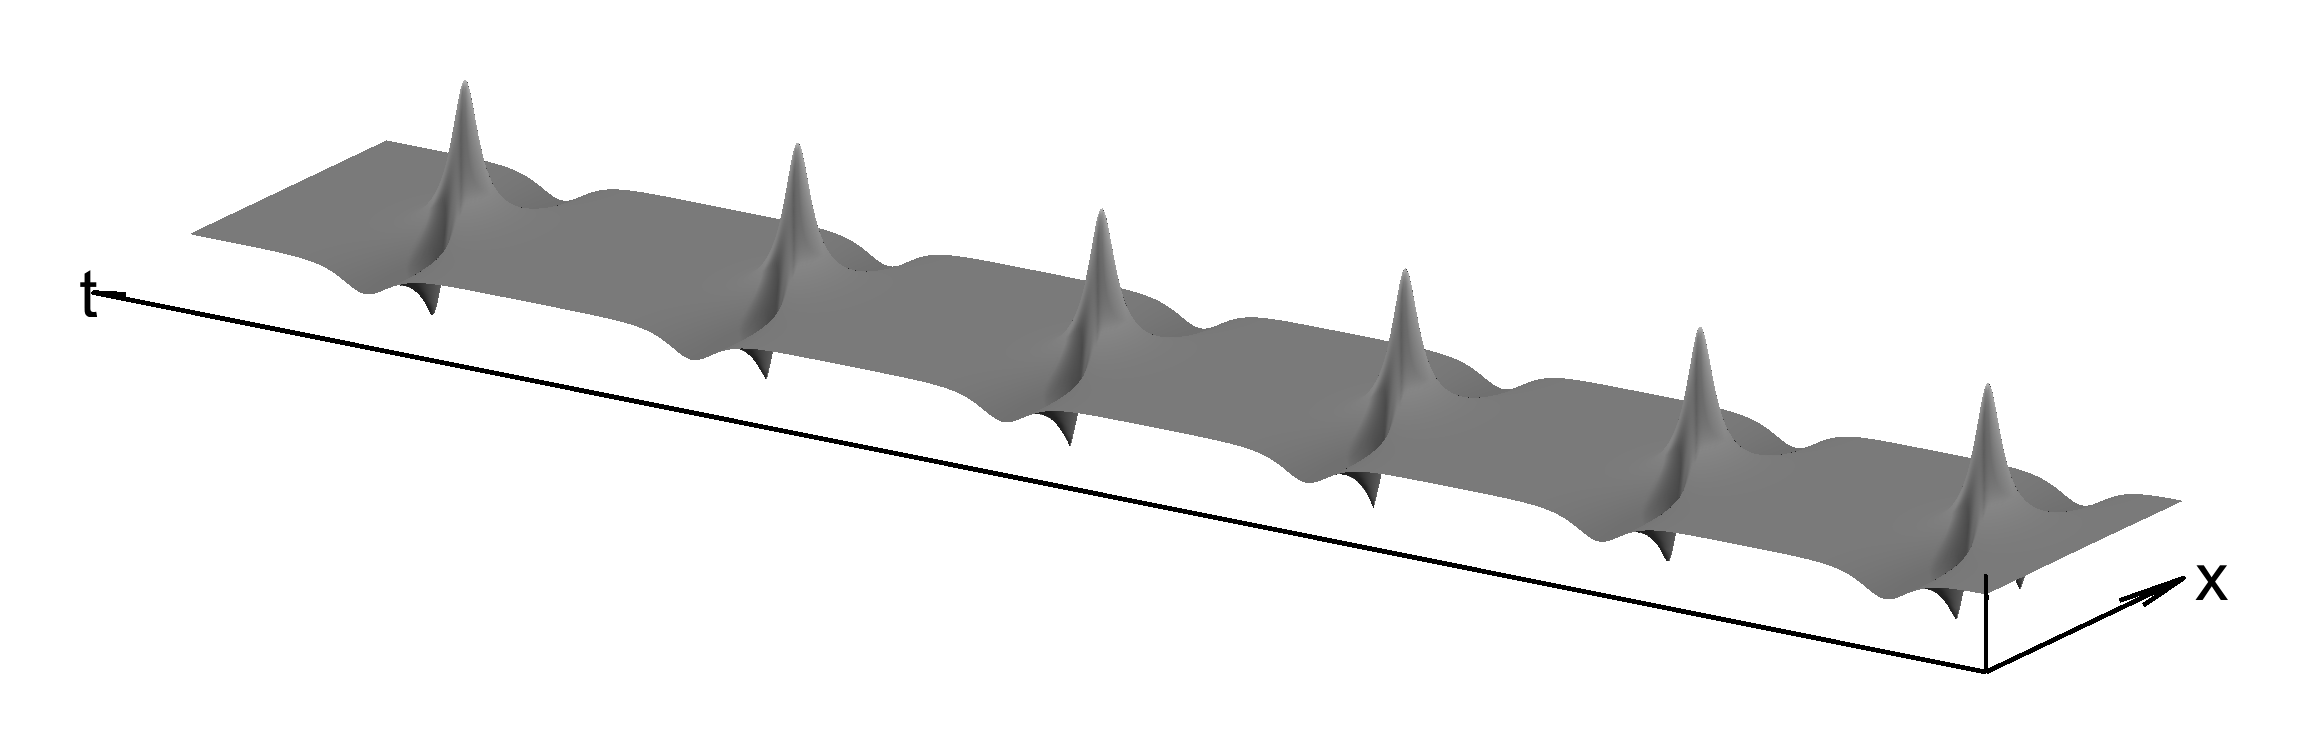
\includegraphics[width=0.88\textwidth]{hw3/paper_fig1_reproduction_bw_v6.png}
\caption{Paper-style black-and-white reproduction produced by
\texttt{reproduce\_paper\_fig1\_bw\_v6.m}.  This version uses the same
split-step Fourier data as before, but crops the MATLAB export so that
the three-dimensional recurrence fills the canvas more effectively while
keeping the same \LaTeX{} figure width.}
\label{fig:hw3-paper-style-v6}
\end{center}

Figure~\ref{fig:hw3-paper-style-v6} shows the expected anomalous-wave
recurrence.  For small \(t\), the surface is close to the background
\(|u|=1\).  The one unstable Fourier mode then grows, a sharp nonlinear
peak forms, and the solution returns close to the background before the
next growth stage.  The important point is that the large peak is not
inserted by hand: it is generated by repeatedly applying the three
Strang-splitting operations described above.

\noteheading{Supplementary views and stability checks.}
The earlier colored view is kept because it gives a complementary way to
read the recurrence times: the nearly uniform background corresponds to
\(|u|\approx 1\), while the localized high-amplitude regions correspond
to the nonlinear peaks in the paper-style surface.  To check that the
large peaks are not merely plotting artifacts, we also ran the same type
of split-step Fourier simulation in two stable regimes.  In the first
stable test, the code keeps a fine grid and small time step, but changes
the length to \(L=2\).  Then
\begin{equation}
k_1=\frac{2\pi}{L}=\pi>2.
\label{eq:hw3-stable-mode}
\end{equation}
Thus the first Fourier mode is outside the modulationally unstable band.
With a small perturbation and conservative numerical parameters, the
solution remains close to the unit background.  The under-resolved test
uses a coarser grid \(N_x=256\), a much larger final time
\(T_{\max}=250\), and only \(N_t=20000\) time steps; its irregular spikes
should therefore be interpreted as numerical drift or accumulated
discretization error, not as physical modulation instability.  The three
checks are collected compactly in Figure~\ref{fig:hw3-supplementary-checks}.

\begin{center}
\captionsetup{type=figure,hypcap=false}
\centering
\setlength{\tabcolsep}{2pt}
\begin{tabular}{ccc}
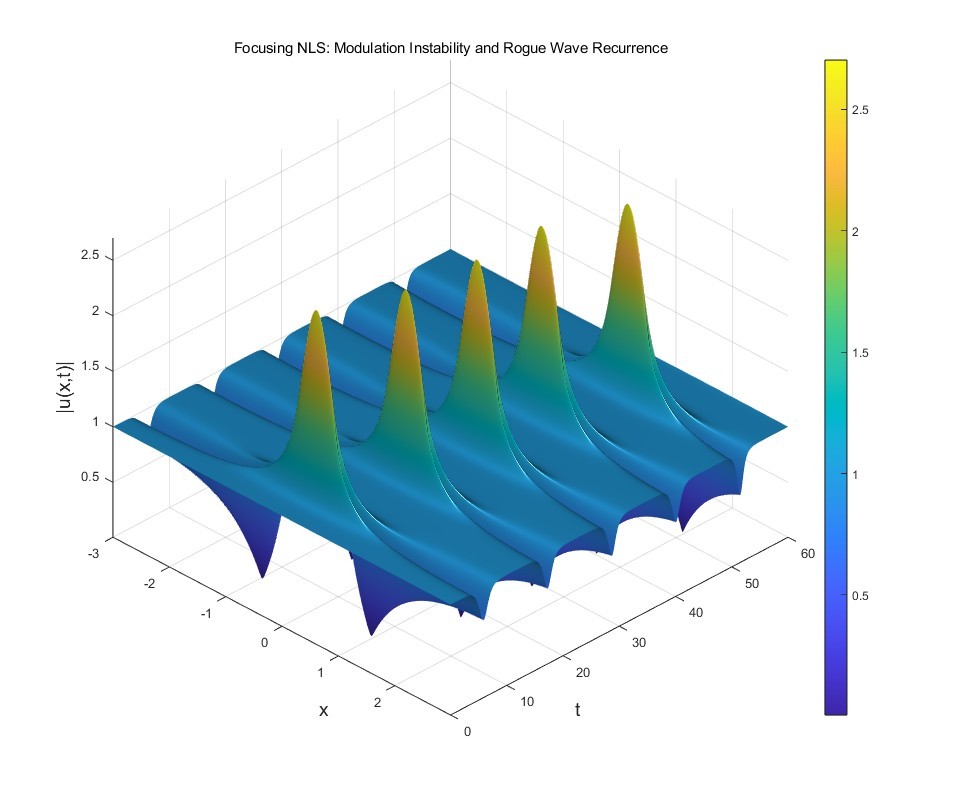
\includegraphics[width=0.315\textwidth,trim=55 70 65 70,clip]{hw3/nls_level_plot_fig1.jpg}
&
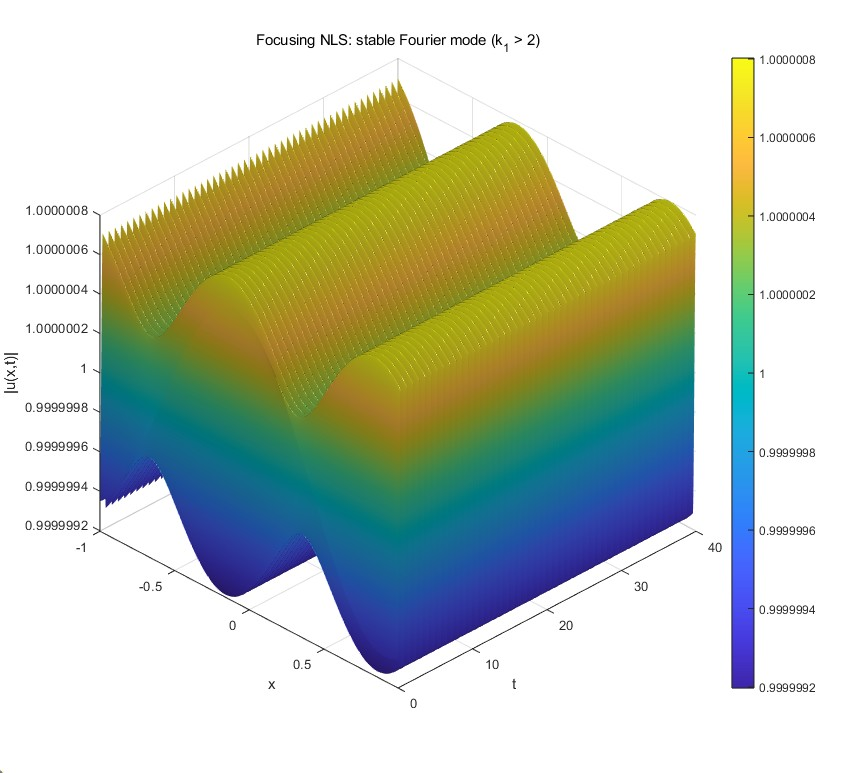
\includegraphics[width=0.315\textwidth,trim=50 70 55 70,clip]{hw3/nls_3d_surface_stable_mode.jpg}
&
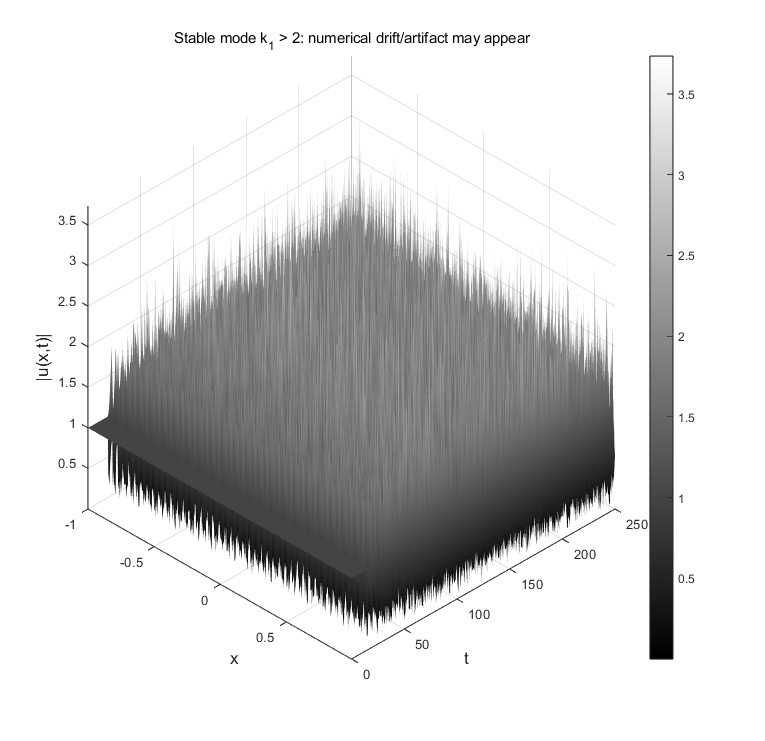
\includegraphics[width=0.315\textwidth,trim=45 65 50 70,clip]{hw3/nls_stable_mode_numerical_artifact_bw.jpg}
\\[-0.2em]
\parbox[t]{0.315\textwidth}{\centering\small (a) Colored recurrence view}
&
\parbox[t]{0.315\textwidth}{\centering\small (b) Stable well-resolved run}
&
\parbox[t]{0.315\textwidth}{\centering\small (c) Under-resolved artifact run}
\end{tabular}
\caption{Supplementary views and stability checks.  Panel (a) gives a
colored view of the one-mode recurrence, panel (b) shows a stable
well-resolved run, and panel (c) shows that coarse long-time simulations
can create spurious peaks even in a stable regime.}
\label{fig:hw3-supplementary-checks}
\end{center}

This compact comparison separates the genuine one-mode recurrence in
Figure~\ref{fig:hw3-paper-style-v6} from artifacts caused by insufficient
numerical resolution.



% \clearpage
% \section*{References}

% \begin{enumerate}

% \item Ling, L. and Sun, X., \emph{Focusing mKdV equation: Two-phase solutions and their stability analysis}, 2025. \url{https://arxiv.org/abs/2510.12073}

% \item Bobenko, A., \emph{Compact Riemann Surfaces}. \url{https://page.math.tu-berlin.de/~bobenko/Lehre/Skripte/RS.pdf}

% \item Bertola, M., \emph{Riemann Surfaces and Theta Functions}. \url{https://mypage.concordia.ca/mathstat/bertola/ThetaCourse/ThetaCourse.pdf}

% \item Taylor, M., \emph{Notes on Compact Riemann Surfaces}. \url{https://mtaylor.web.unc.edu/wp-content/uploads/sites/16915/2018/04/RSURF.pdf}

% % \item 王竹溪, 郭敦仁, \emph{特殊函数概论}, 北京大学出版社, 2012.

% % \item 吴崇试, \emph{特殊函数概论习题解答}, 北京大学出版社.

% \item Simon, B., \emph{Basic Complex Analysis}, American Mathematical Society, Part 2A, 2015.

% \item Belokolos, E. D., Bobenko, A. I., Enolskii, V. Z., Its, A. R., Matveev, V. B., \emph{Algebro-Geometric Approach to Nonlinear Integrable Equations}, Springer, 1994.

% \item Gesztesy, F., Holden, H., \emph{Soliton Equations and Their Algebro-Geometric Solutions}, Cambridge University Press, 2003.

% \end{enumerate}

% \bibliographystyle{plainurl}
% \nocite{*}          % include all BibTeX entries
% \bibliography{references}  




% \bibliographystyle{siam}
% \bibliography{CFL-pattern}





\end{document}
